\documentclass[11pt,fleqn, openany]{book} % Default font size and left-justified equations

%%%%%%%%%%%%%%%%%%%%%%%%%%%%%%%%%%%%%%%%%
% The Legrand Orange Book
% Structural Definitions File
% Version 2.1 (26/09/2018)
%
% Original author:
% Mathias Legrand (legrand.mathias@gmail.com) with modifications by:
% Vel (vel@latextemplates.com)
% 
% This file was downloaded from:
% http://www.LaTeXTemplates.com
%
% License:
% CC BY-NC-SA 3.0 (http://creativecommons.org/licenses/by-nc-sa/3.0/)
%
%%%%%%%%%%%%%%%%%%%%%%%%%%%%%%%%%%%%%%%%%

%----------------------------------------------------------------------------------------
%	VARIOUS REQUIRED PACKAGES AND CONFIGURATIONS
%----------------------------------------------------------------------------------------

\usepackage[table]{xcolor}

\usepackage{graphicx}
\usepackage{tabularx} % Required for including pictures
\usepackage{pgf,tikz,tkz-tab,eurosym,yhmath, stmaryrd}
\usepackage{pgfplots}
\usepackage{mathrsfs}
\usetikzlibrary{patterns}
\usetikzlibrary{trees}
\graphicspath{{../../Pictures/}}
\usepackage{multicol} 


\usepackage[english]{babel} % English language/hyphenation
\usepackage{icomma}
\usepackage{enumitem} % Customize lists
\setlist{nolistsep, nosep, nolistsep} % Reduce spacing between bullet points and numbered lists

\usepackage{booktabs} % Required for nicer horizontal rules in tables

 % Required for specifying colors by name


\definecolor{ocre}{RGB}{243,102,25} % Define the orange color used for highlighting throughout the book

\usepackage{listings}

\definecolor{codegreen}{rgb}{0,0.6,0}
\definecolor{codegray}{rgb}{0.5,0.5,0.5}
\definecolor{codepurple}{rgb}{0.58,0,0.82}
\definecolor{backcolour}{rgb}{0.95,0.95,0.92}

\lstdefinestyle{mystyle}{
    backgroundcolor=\color{backcolour},   
    commentstyle=\color{codegreen},
    keywordstyle=\color{magenta},
    numberstyle=\tiny\color{codegray},
    stringstyle=\color{codepurple},
    basicstyle=\ttfamily\footnotesize,
    breakatwhitespace=false,         
    breaklines=true,                 
    captionpos=b,                    
    keepspaces=true,                 
    numbers=left,                    
    numbersep=5pt,                  
    showspaces=false,                
    showstringspaces=false,
    showtabs=false,                  
    tabsize=2
}

\lstset{style=mystyle}

%----------------------------------------------------------------------------------------
% Paramétrage XSIM
%----------------------------------------------------------------------------------------

\usepackage[no-files]{xsim}


\DeclareExerciseEnvironmentTemplate{myex}{%
    \textbf{%
      \hypertarget{ex:\ExerciseID}{\sffamily{\ensuremath{\blacktriangleright}} Exercice \GetExerciseProperty{counter} \GetExerciseProperty{subtitle} --}
      \hyperlink{sol:\ExerciseID}{Voir le corrigé}%
    }\par
}{\par\smallskip}

\DeclareExerciseEnvironmentTemplate{mysol}{%
    \textbf{%
      \hypertarget{sol:\ExerciseID}{\sffamily{\ensuremath{\blacktriangleright}} Correction \GetExerciseProperty{counter} --}
      \hyperlink{ex:\ExerciseID}{Voir l'énoncé}%
    }\par
}{\par\medskip}

\xsimsetup{
  exercise/template = myex ,
  solution/template = mysol 
}

%Collection exercices

\DeclareExerciseTagging{topic}

\xsimsetup{collect}

%----------------------------------------------------------------------------------------
% SYMBOLES
%----------------------------------------------------------------------------------------

\newcommand\imCMsym[4][\mathord]{%
  \DeclareFontFamily{U} {#2}{}
  \DeclareFontShape{U}{#2}{m}{n}{
    <-6> #25
    <6-7> #26
    <7-8> #27
    <8-9> #28
    <9-10> #29
    <10-12> #210
    <12-> #212}{}
  \DeclareSymbolFont{CM#2} {U} {#2}{m}{n}
  \DeclareMathSymbol{#4}{#1}{CM#2}{#3}
}
\newcommand\alsoimCMsym[4][\mathord]{\DeclareMathSymbol{#4}{#1}{CM#2}{#3}}

\imCMsym{cmmi}{124}{\CMjmath}

\newcommand{\Oij}{(O\,;\,\vec{\imath}\,,\, \vec{\CMjmath} )}
\newcommand{\Oijk}{(O\,;\,\vec{\imath}\,,\, \vec{\CMjmath}\,,\,\vec{k})}

\newcommand\e{\mathrm{e}}
\newcommand\R{\mathbb{R}}
\newcommand\N{\mathbb{N}}


%----------------------------------------------------------------------------------------
%	MARGINS
%----------------------------------------------------------------------------------------

\usepackage{geometry} % Required for adjusting page dimensions and margins

\geometry{
	paper=a4paper, % Paper size, change to letterpaper for US letter size
	top=3cm, % Top margin
	bottom=3cm, % Bottom margin
	left=2cm, % Left margin
	right=2cm, % Right margin
	headheight=14pt, % Header height
	footskip=1.4cm, % Space from the bottom margin to the baseline of the footer
	headsep=10pt, % Space from the top margin to the baseline of the header
	%showframe, % Uncomment to show how the type block is set on the page
}

\setlength{\parindent}{0pt}
\parskip=5pt



%----------------------------------------------------------------------------------------
%	FONTS
%----------------------------------------------------------------------------------------

\usepackage{avant} % Use the Avantgarde font for headings
\usepackage{times} % Use the Times font for headings
\usepackage{mathptmx} % Use the Adobe Times Roman as the default text font together with math symbols from the Sym­bol, Chancery and Com­puter Modern fonts

%\usepackage{microtype} % Slightly tweak font spacing for aesthetics
%\usepackage[utf8]{inputenc} % Required for including letters with accents
\usepackage[T1]{fontenc} % Use 8-bit encoding that has 256 glyphs

%----------------------------------------------------------------------------------------
%	BIBLIOGRAPHY AND INDEX
%----------------------------------------------------------------------------------------

\usepackage[style=numeric,citestyle=numeric,sorting=nyt,sortcites=true,autopunct=true,babel=hyphen,hyperref=true,abbreviate=false,backref=true,backend=biber]{biblatex}
\addbibresource{bibliography.bib} % BibTeX bibliography file
\defbibheading{bibempty}{}

\usepackage{calc} % For simpler calculation - used for spacing the index letter headings correctly
\usepackage{makeidx} % Required to make an index
\makeindex % Tells LaTeX to create the files required for indexing

%----------------------------------------------------------------------------------------
%	MAIN TABLE OF CONTENTS
%----------------------------------------------------------------------------------------

\usepackage{titletoc} % Required for manipulating the table of contents

\contentsmargin{0cm} % Removes the default margin

% Part text styling (this is mostly taken care of in the PART HEADINGS section of this file)
\titlecontents{part}
	[0cm] % Left indentation
	{\addvspace{20pt}\bfseries} % Spacing and font options for parts
	{}
	{}
	{}

% Chapter text styling
\titlecontents{chapter}
	[1.25cm] % Left indentation
	{\addvspace{12pt}\large\sffamily\bfseries} % Spacing and font options for chapters
	{\color{ocre!60}\contentslabel[\Large\thecontentslabel]{1.25cm}\color{ocre}} % Formatting of numbered sections of this type
	{\color{ocre}} % Formatting of numberless sections of this type
	{\color{ocre!60}\normalsize\;\titlerule*[.5pc]{.}\;\thecontentspage} % Formatting of the filler to the right of the heading and the page number

% Section text styling
\titlecontents{section}
	[1.25cm] % Left indentation
	{\addvspace{3pt}\sffamily\bfseries} % Spacing and font options for sections
	{\contentslabel[\thecontentslabel]{1.25cm}} % Formatting of numbered sections of this type
	{} % Formatting of numberless sections of this type
	{\hfill\color{black}\thecontentspage} % Formatting of the filler to the right of the heading and the page number

% Subsection text styling
\titlecontents{subsection}
	[1.25cm] % Left indentation
	{\addvspace{1pt}\sffamily\small} % Spacing and font options for subsections
	{\contentslabel[\thecontentslabel]{1.25cm}} % Formatting of numbered sections of this type
	{} % Formatting of numberless sections of this type
	{\ \titlerule*[.5pc]{.}\;\thecontentspage} % Formatting of the filler to the right of the heading and the page number

% Figure text styling
\titlecontents{figure}
	[1.25cm] % Left indentation
	{\addvspace{1pt}\sffamily\small} % Spacing and font options for figures
	{\thecontentslabel\hspace*{1em}} % Formatting of numbered sections of this type
	{} % Formatting of numberless sections of this type
	{\ \titlerule*[.5pc]{.}\;\thecontentspage} % Formatting of the filler to the right of the heading and the page number

% Table text styling
\titlecontents{table}
	[1.25cm] % Left indentation
	{\addvspace{1pt}\sffamily\small} % Spacing and font options for tables
	{\thecontentslabel\hspace*{1em}} % Formatting of numbered sections of this type
	{} % Formatting of numberless sections of this type
	{\ \titlerule*[.5pc]{.}\;\thecontentspage} % Formatting of the filler to the right of the heading and the page number

%----------------------------------------------------------------------------------------
%	MINI TABLE OF CONTENTS IN PART HEADS
%----------------------------------------------------------------------------------------

% Chapter text styling
\titlecontents{lchapter}
	[0em] % Left indentation
	{\addvspace{15pt}\large\sffamily\bfseries} % Spacing and font options for chapters
	{\color{ocre}\contentslabel[\Large\thecontentslabel]{1.25cm}\color{ocre}} % Chapter number
	{}  
	{\color{ocre}\normalsize\sffamily\bfseries\;\titlerule*[.5pc]{.}\;\thecontentspage} % Page number

% Section text styling
\titlecontents{lsection}
	[0em] % Left indentation
	{\sffamily\small} % Spacing and font options for sections
	{\contentslabel[\thecontentslabel]{1.25cm}} % Section number
	{}
	{}

% Subsection text styling (note these aren't shown by default, display them by searchings this file for tocdepth and reading the commented text)
\titlecontents{lsubsection}
	[.5em] % Left indentation
	{\sffamily\footnotesize} % Spacing and font options for subsections
	{\contentslabel[\thecontentslabel]{1.25cm}}
	{}
	{}

%----------------------------------------------------------------------------------------
%	HEADERS AND FOOTERS
%----------------------------------------------------------------------------------------


\usepackage{fancyhdr} % Required for header and footer configuration

\pagestyle{fancy}
\renewcommand{\chaptermark}[1]{\markboth{\sffamily\normalsize\bfseries\ \thechapter.\ #1}{}} % Chapter text font settings
\renewcommand{\sectionmark}[1]{\markright{\sffamily\normalsize\thesection\hspace{5pt}#1}{}} % Section text font settings
\fancyhf{} \fancyhead[LE,RO]{\sffamily\normalsize\thepage} % Font setting for the page number in the header
\fancyhead[LO]{\rightmark} % Print the nearest section name on the left side of odd pages
\fancyhead[RE]{\leftmark} % Print the current chapter name on the right side of even pages

\fancyfoot[L]{Jason LAPEYRONNIE}
\fancyfoot[R]{\href{http://mathoutils.fr}{http://mathoutils.fr}} % Uncomment to include a footer

\renewcommand{\headrulewidth}{0.5pt} % Thickness of the rule under the header
\renewcommand{\footrulewidth}{0.5pt} % Thickness of the rule under the header

\fancypagestyle{plain}{% Style for when a plain pagestyle is specified
	\fancyhead{}\renewcommand{\headrulewidth}{0pt}%
}

% Removes the header from odd empty pages at the end of chapters
\makeatletter
\renewcommand{\cleardoublepage}{
\clearpage\ifodd\c@page\else
\hbox{}
\vspace*{\fill}
\thispagestyle{empty}
\newpage
\fi}

%----------------------------------------------------------------------------------------
%	THEOREM STYLES
%----------------------------------------------------------------------------------------

\usepackage{amsmath,amsfonts,amssymb,amsthm} % For math equations, theorems, symbols, etc

\newcommand{\intoo}[2]{\mathopen{]}#1\,;#2\mathclose{[}}
\newcommand{\ud}{\mathop{\mathrm{{}d}}\mathopen{}}
\newcommand{\intff}[2]{\mathopen{[}#1\,;#2\mathclose{]}}
\renewcommand{\qedsymbol}{$\blacksquare$}
\newtheorem{notation}{Notation}[section]

% Boxed/framed environments
\newtheoremstyle{ocrenumbox}% Theorem style name
{0pt}% Space above
{0pt}% Space below
{\normalfont}% Body font
{}% Indent amount
{\small\bf\sffamily\color{ocre}}% Theorem head font
{\;:\;}% Punctuation after theorem head
{0.25em}% Space after theorem head
{\small\sffamily\color{ocre}\thmname{#1}\nobreakspace\thmnumber{\@ifnotempty{#1}{}\@upn{#2}}% Theorem text (e.g. Theorem 2.1)
\thmnote{\nobreakspace\the\thm@notefont\sffamily\bfseries\color{black}---\nobreakspace#3}} % Optional theorem note

\newtheoremstyle{blacknumex}% Theorem style name
{5pt}% Space above
{10pt}% Space below
{\normalfont}% Body font
{} % Indent amount
{\small\bf\sffamily}% Theorem head font
{\;:\;}% Punctuation after theorem head
{0.25em}% Space after theorem head
{\small\sffamily{\tiny\ensuremath{\blacksquare}}\nobreakspace\thmname{#1}\nobreakspace\thmnumber{\@ifnotempty{#1}{}\@upn{#2}}% Theorem text (e.g. Theorem 2.1)
\thmnote{\nobreakspace\the\thm@notefont\sffamily\bfseries---\nobreakspace#3}}% Optional theorem note

\newtheoremstyle{blacknumexo}% Theorem style name
{15pt}% Space above
{10pt}% Space below
{\normalfont}% Body font
{} % Indent amount
{\small\bf\sffamily}% Theorem head font
{}% Punctuation after theorem head
{0.5em}% Space after theorem head
{\small\sffamily{\ensuremath{\blacktriangleright}}\nobreakspace\thmname{#1}\nobreakspace\thmnumber{\@ifnotempty{#1}{}\@upn{#2}}% Theorem text (e.g. Theorem 2.1)
\thmnote{\nobreakspace\the\thm@notefont\sffamily\bfseries---\nobreakspace#3} \\}% Optional theorem note



\newtheoremstyle{blacknumbox} % Theorem style name
{0pt}% Space above
{5pt}% Space below
{}% Body font
{}% Indent amount
{\large\bf\sffamily}% Theorem head font
{\;:\;}% Punctuation after theorem head
{0.25em}% Space after theorem head
{\small\sffamily\thmname{#1}\nobreakspace\thmnumber{\@ifnotempty{#1}{}\@upn{#2}}% Theorem text (e.g. Theorem 2.1)
\thmnote{\nobreakspace\the\thm@notefont\sffamily\bfseries---\nobreakspace#3}}% Optional theorem note

% Non-boxed/non-framed environments
\newtheoremstyle{ocrenum}% Theorem style name
{5pt}% Space above
{5pt}% Space below
{\normalfont}% Body font
{}% Indent amount
{\small\bf\sffamily\color{ocre}}% Theorem head font
{\;:\;}% Punctuation after theorem head
{0.25em}% Space after theorem head
{\small\sffamily\color{ocre}\thmname{#1}\nobreakspace\thmnumber{\@ifnotempty{#1}{}\@upn{#2}}% Theorem text (e.g. Theorem 2.1)
\thmnote{\nobreakspace\the\thm@notefont\sffamily\bfseries\color{black}---\nobreakspace#3}} % Optional theorem note
\makeatother

% Defines the theorem text style for each type of theorem to one of the three styles above
\newcounter{dummy} 
\newcounter{thm}
\newcounter{correction}
\newcounter{qst}
\theoremstyle{ocrenumbox}
\newtheorem{theoremeT}[dummy]{Théorème}
\newtheorem{exerciseT}{Propriété}
\newtheorem{principeT}{Principe}
\theoremstyle{blacknumex}
\newtheorem{exampleT}{Exemple}
\theoremstyle{blacknumexo}
\newtheorem{exo}[thm]{Exercice}
\newtheorem{corr}[correction]{Correction}
\newtheorem{quest}[qst]{Question}
\theoremstyle{blacknumbox}
\newtheorem{vocabulary}{Vocabulary}[section]
\newtheorem{definitionT}{Définition}
\newtheorem{corollaryT}[dummy]{Corollary}
\theoremstyle{ocrenum}
\newtheorem{proofT}[dummy]{Démonstration}


%----------------------------------------------------------------------------------------
%	DEFINITION OF COLORED BOXES
%----------------------------------------------------------------------------------------

\RequirePackage[framemethod=default]{mdframed} % Required for creating the theorem, definition, exercise and corollary boxes

% Theorem box
\newmdenv[skipabove=7pt,
skipbelow=7pt,
backgroundcolor=black!5,
linecolor=ocre,
innerleftmargin=5pt,
innerrightmargin=5pt,
innertopmargin=10pt,
leftmargin=0cm,
rightmargin=0cm,
innerbottommargin=5pt]{tBox}

%Proposition box	  
\newmdenv[skipabove=7pt,
skipbelow=7pt,
rightline=false,
leftline=true,
topline=false,
bottomline=false,
backgroundcolor=ocre!10,
linecolor=ocre,
innerleftmargin=5pt,
innerrightmargin=5pt,
innertopmargin=10pt,
innerbottommargin=3pt,
leftmargin=0cm,
rightmargin=0cm,
linewidth=4pt]{eBox}	

% Definition box
\newmdenv[skipabove=7pt,
backgroundcolor=ocre!4,
skipbelow=7pt,
rightline=false,
leftline=true,
topline=false,
bottomline=false,
linecolor=ocre,
innerleftmargin=5pt,
innerrightmargin=5pt,
innertopmargin=10pt,
leftmargin=0cm,
rightmargin=0cm,
linewidth=4pt,
innerbottommargin=5pt]{dBox}	

% Corollary box
\newmdenv[skipabove=7pt,
skipbelow=7pt,
rightline=false,
leftline=true,
topline=false,
bottomline=false,
linecolor=gray,
backgroundcolor=black!5,
innerleftmargin=5pt,
innerrightmargin=5pt,
innertopmargin=5pt,
leftmargin=0cm,
rightmargin=0cm,
linewidth=4pt,
innerbottommargin=5pt]{cBox}

\newmdenv[skipabove=7pt,
skipbelow=7pt,
backgroundcolor=black!5,
innerleftmargin=5pt,
topline=false,
bottomline=false,
rightline=false,
leftline=false,
innerrightmargin=5pt,
innertopmargin=5pt,
leftmargin=0cm,
rightmargin=0cm,
innerbottommargin=5pt]{xBox}

% Creates an environment for each type of theorem and assigns it a theorem text style from the "Theorem Styles" section above and a colored box from above
\newenvironment{theorem}{\begin{tBox}\begin{theoremeT}}{\end{theoremeT}\end{tBox}}

\newenvironment{exo2}{\noindent \begin{exo}\item\relax \noindent \begin{eBox}\item\relax}{\end{eBox}\end{exo}}


\newenvironment{proposition}{\begin{eBox}\begin{exerciseT}}{\hfill{\color{ocre}}\end{exerciseT}\end{eBox}}		

\newenvironment{principe}{\begin{eBox}\begin{principeT}}{\hfill{\color{ocre}}\end{principeT}\end{eBox}}	
		  
\newenvironment{definition}{\begin{dBox}\begin{definitionT}}{\end{definitionT}\end{dBox}}	

\newenvironment{example}{\begin{xBox}\begin{exampleT}}{\hfill{\tiny\ensuremath{\blacksquare}}\end{exampleT}\end{xBox}}

\newenvironment{demonstration}{\begin{proofT}}{\hfill{\tiny\ensuremath{\square}}\end{proofT}}		
\newenvironment{corollary}{\begin{cBox}\begin{corollaryT}}{\end{corollaryT}\end{cBox}}	

%----------------------------------------------------------------------------------------
%	REMARK ENVIRONMENT
%----------------------------------------------------------------------------------------

\newenvironment{remark}{\par\vspace{5pt}\small % Vertical white space above the remark and smaller font size
\begin{list}{}{
\leftmargin=25pt % Indentation on the left
\rightmargin=15pt}\item\ignorespaces % Indentation on the right
\makebox[-2.5pt]{\begin{tikzpicture}[overlay]
\node[draw=ocre!60,line width=1pt,circle,fill=ocre!25,font=\sffamily\bfseries,inner sep=2pt,outer sep=0pt] at (-15pt,0pt){\textcolor{ocre}{R}};\end{tikzpicture}} % Orange R in a circle
\advance\baselineskip -1pt}{\end{list}\vskip5pt} % Tighter line spacing and white space after remark

%----------------------------------------------------------------------------------------
%	SECTION NUMBERING IN THE MARGIN
%----------------------------------------------------------------------------------------

\makeatletter
\renewcommand{\@seccntformat}[1]{\llap{\textcolor{ocre}{\csname the#1\endcsname}\hspace{1em}}}                    
\renewcommand{\section}{\@startsection{section}{1}{\z@}
{-4ex \@plus -1ex \@minus -.4ex}
{1ex \@plus.2ex }
{\normalfont\LARGE\sffamily\bfseries}}
\renewcommand{\subsection}{\@startsection {subsection}{2}{\z@}
{-3ex \@plus -0.1ex \@minus -.4ex}
{0.5ex \@plus.2ex }
{\normalfont\sffamily\bfseries}}
\renewcommand{\subsubsection}{\@startsection {subsubsection}{3}{\z@}
{-2ex \@plus -0.1ex \@minus -.2ex}
{.2ex \@plus.2ex }
{\normalfont\small\sffamily\bfseries}}                        
\renewcommand\paragraph{\@startsection{paragraph}{4}{\z@}
{-2ex \@plus-.2ex \@minus .2ex}
{.1ex}
{\normalfont\small\sffamily\bfseries}}

%----------------------------------------------------------------------------------------
%	PART HEADINGS
%----------------------------------------------------------------------------------------

% Numbered part in the table of contents
\newcommand{\@mypartnumtocformat}[2]{%
	\setlength\fboxsep{0pt}%
	\noindent\colorbox{ocre!20}{\strut\parbox[c][.7cm]{\ecart}{\color{ocre!70}\Large\sffamily\bfseries\centering#1}}\hskip\esp\colorbox{ocre!40}{\strut\parbox[c][.7cm]{\linewidth-\ecart-\esp}{\Large\sffamily\centering#2}}%
}

% Unnumbered part in the table of contents
\newcommand{\@myparttocformat}[1]{%
	\setlength\fboxsep{0pt}%
	\noindent\colorbox{ocre!40}{\strut\parbox[c][.7cm]{\linewidth}{\Large\sffamily\centering#1}}%
}

\newlength\esp
\setlength\esp{4pt}
\newlength\ecart
\setlength\ecart{1.2cm-\esp}
\newcommand{\thepartimage}{}%
\newcommand{\partimage}[1]{\renewcommand{\thepartimage}{#1}}%
\def\@part[#1]#2{%
\ifnum \c@secnumdepth >-2\relax%
\refstepcounter{part}%
\addcontentsline{toc}{part}{\texorpdfstring{\protect\@mypartnumtocformat{\thepart}{#1}}{\partname~\thepart\ ---\ #1}}
\else%
\addcontentsline{toc}{part}{\texorpdfstring{\protect\@myparttocformat{#1}}{#1}}%
\fi%
\startcontents%
\markboth{}{}%
{\thispagestyle{empty}%
\begin{tikzpicture}[remember picture,overlay]%
\node at (current page.north west){\begin{tikzpicture}[remember picture,overlay]%	
\fill[ocre!20](0cm,0cm) rectangle (\paperwidth,-\paperheight);
\node[anchor=north] at (4cm,-3.25cm){\color{ocre!40}\fontsize{220}{100}\sffamily\bfseries\thepart}; 
\node[anchor=south east] at (\paperwidth-1cm,-\paperheight+1cm){\parbox[t][][t]{8.5cm}{
\printcontents{l}{0}{\setcounter{tocdepth}{1}}% The depth to which the Part mini table of contents displays headings; 0 for chapters only, 1 for chapters and sections and 2 for chapters, sections and subsections
}};
\node[anchor=north east] at (\paperwidth-1.5cm,-3.25cm){\parbox[t][][t]{15cm}{\strut\raggedleft\color{white}\fontsize{30}{30}\sffamily\bfseries#2}};
\end{tikzpicture}};
\end{tikzpicture}}%
\@endpart}
\def\@spart#1{%
\startcontents%
\phantomsection
{\thispagestyle{empty}%
\begin{tikzpicture}[remember picture,overlay]%
\node at (current page.north west){\begin{tikzpicture}[remember picture,overlay]%	
\fill[ocre!20](0cm,0cm) rectangle (\paperwidth,-\paperheight);
\node[anchor=north east] at (\paperwidth-1.5cm,-3.25cm){\parbox[t][][t]{15cm}{\strut\raggedleft\color{white}\fontsize{30}{30}\sffamily\bfseries#1}};
\end{tikzpicture}};
\end{tikzpicture}}
\addcontentsline{toc}{part}{\texorpdfstring{%
\setlength\fboxsep{0pt}%
\noindent\protect\colorbox{ocre!40}{\strut\protect\parbox[c][.7cm]{\linewidth}{\Large\sffamily\protect\centering #1\quad\mbox{}}}}{#1}}%
\@endpart}
\def\@endpart{\vfil\newpage
\if@twoside
\if@openright
\null
\thispagestyle{empty}%
\newpage
\fi
\fi
\if@tempswa
\twocolumn
\fi}

%----------------------------------------------------------------------------------------
%	CHAPTER HEADINGS
%----------------------------------------------------------------------------------------

% A switch to conditionally include a picture, implemented by Christian Hupfer
\newif\ifusechapterimage
\usechapterimagetrue
\newcommand{\thechapterimage}{}%
\newcommand{\chapterimage}[1]{\ifusechapterimage\renewcommand{\thechapterimage}{#1}\fi}%
\newcommand{\autodot}{.}
\def\@makechapterhead#1{%
{\parindent \z@ \raggedright \normalfont
\ifnum \c@secnumdepth >\m@ne
\if@mainmatter
\begin{tikzpicture}[remember picture,overlay]
\node at (current page.north west)
{\begin{tikzpicture}[remember picture,overlay]
\node[anchor=north west,inner sep=0pt] at (0,0) {\ifusechapterimage\includegraphics[width=\paperwidth]{\thechapterimage}\fi};
\draw[anchor=west] (\Gm@lmargin,-3cm) node [line width=2pt,rounded corners=15pt,draw=ocre,fill=white,fill opacity=0.5,inner sep=15pt]{\strut\makebox[22cm]{}};
\draw[anchor=west] (\Gm@lmargin+.3cm,-3cm) node {\huge\sffamily\bfseries\color{black}\thechapter\autodot~#1\strut};
\end{tikzpicture}};
\end{tikzpicture}
\else
\begin{tikzpicture}[remember picture,overlay]
\node at (current page.north west)
{\begin{tikzpicture}[remember picture,overlay]
\node[anchor=north west,inner sep=0pt] at (0,0) {\ifusechapterimage\includegraphics[width=\paperwidth]{\thechapterimage}\fi};
\draw[anchor=west] (\Gm@lmargin,-3cm) node [line width=2pt,rounded corners=15pt,draw=ocre,fill=white,fill opacity=0.5,inner sep=15pt]{\strut\makebox[22cm]{}};
\draw[anchor=west] (\Gm@lmargin+.3cm,-3cm) node {\huge\sffamily\bfseries\color{black}#1\strut};
\end{tikzpicture}};
\end{tikzpicture}
\fi\fi\par\vspace*{50\p@}}}

%-------------------------------------------

\def\@makeschapterhead#1{%
\begin{tikzpicture}[remember picture,overlay]
\node at (current page.north west)
{\begin{tikzpicture}[remember picture,overlay]
\node[anchor=north west,inner sep=0pt] at (0,0) {\ifusechapterimage\includegraphics[width=\paperwidth]{\thechapterimage}\fi};
\draw[anchor=west] (\Gm@lmargin,-3cm) node [line width=2pt,rounded corners=15pt,draw=ocre,fill=white,fill opacity=0.5,inner sep=15pt]{\strut\makebox[22cm]{}};
\draw[anchor=west] (\Gm@lmargin+.3cm,-3cm) node {\huge\sffamily\bfseries\color{black}#1\strut};
\end{tikzpicture}};
\end{tikzpicture}
\par\vspace*{50\p@}}
\makeatother

%----------------------------------------------------------------------------------------
%	LINKS
%----------------------------------------------------------------------------------------

\usepackage{hyperref}
\hypersetup{hidelinks,backref=true,pagebackref=true,hyperindex=true,colorlinks=false,breaklinks=true,urlcolor=ocre,bookmarks=true,bookmarksopen=false}

\usepackage{bookmark}
\bookmarksetup{
open,
numbered,
addtohook={%
\ifnum\bookmarkget{level}=0 % chapter
\bookmarksetup{bold}%
\fi
\ifnum\bookmarkget{level}=-1 % part
\bookmarksetup{color=ocre,bold}%
\fi
}
}

\renewcommand*\thesection{\arabic{section}}

\newcommand*{\coord}[3]{% 
  \ensuremath{\overrightarrow{#1}\, 
    \begin{pmatrix} 
      #2\\ 
      #3 
    \end{pmatrix}}}
    
  \newcommand*{\coordb}[2]{% 
  \ensuremath{ 
    \begin{pmatrix} 
      #1\\ 
      #2 
    \end{pmatrix}}}

\newcommand*{\coorde}[4]{% 
  \renewcommand{\arraystretch}{1}\ensuremath{\overrightarrow{#1}\, 
    \begin{pmatrix} 
      #2\\ 
      #3 \\
      #4
    \end{pmatrix}}}    
  \newcommand*{\coordbe}[3]{% 
 \renewcommand{\arraystretch}{1} \ensuremath{ 
    \begin{pmatrix} 
      #1\\ 
      #2 \\
      #3
    \end{pmatrix}}}  
    
\newcommand{\Card}{\mathrm{Card}}



\begin{document}

\chapterimage{../../Pictures/background}


\chapter{Exercices}


\section*{Théorèmes de comparaison et d'encadrement}

\begin{exercise}On considère la suite $(u_n)$ définie pour tout entier naturel $n$ par $u_n=((-1)^n-4)n^2$.
\begin{enumerate}
\item Montrer que pour tout entier naturel $n$, on a $u_n \leqslant -3n^2$.
\item En déduire la limite de $(u_n)$ en $+\infty$.
\end{enumerate}\end{exercise}

\begin{solution}Pour tout entier naturel $n$, on a $-1 \leqslant (-1)^n \leqslant 1$. 

Ainsi, $-1-4 \leqslant (-1)^n -4\leqslant 1-4$, et donc $-5 \leqslant (-1)^n-4 \leqslant -3$.

En multipliant par $n^2$ qui est positif, on a $-5n^2 \leqslant u_n \leqslant -3n^2$.

Puisque $\displaystyle\lim_{n \to + \infty} (-3n^2)=-\infty$, on a, par comparaison, $\displaystyle\lim_{n \to + \infty}u_n=-\infty$.\end{solution}




\begin{exercise}On considère la suite $(u_n)$ définie pour tout entier naturel $n$ par $u_n=\sqrt{n^2+1}$.
\begin{enumerate}
\item Montrer que pour tout entier naturel $n$, on a $u_n \geqslant n$.
\item En déduire la limite de $u_n$ en $+\infty$.
\end{enumerate}\end{exercise}

\begin{solution}Pour tout entier naturel $n$, on a $n^2+1 \geqslant n^2$. En appliquant la fonction Racine carrée qui est croissante sur $[0;+\infty[$, on a alors $\sqrt{n^2+1} \geqslant \sqrt{n^2}$, c'est-à-dire $u_n \geqslant n$.

Puisque $\displaystyle\lim_{n \to + \infty} n=+\infty$, on a, par comparaison, $\displaystyle\lim_{n \to + \infty}u_n=+\infty$.\end{solution}




\begin{exercise}À l'aide d'une majoration ou d'une minoration par une autre suite, déterminer la limite de la suite $(u_n)$ dans chacun des cas suivants.
\renewcommand{\arraystretch}{2.2}
\begin{center}
\begin{tabularx}{\linewidth}{XXXX}
\textbf{a.} $ u_n = n+3\times (-1)^n$ & \textbf{b.} $ u_n=n\,(\sin(n)-3)$ \\
\textbf{c.} $ u_n = n+\dfrac{\cos(n)}{n}$ pour $n>0$ & \textbf{d.} $u_n=\sin(3n^2+1)-n^3$ \\
\end{tabularx}
\end{center}\end{exercise}

\begin{solution}\textbf{a.} Pour tout entier naturel $n$, $u_n=n+3\times (-1)^n$.\\ Or, $-1 \leqslant (-1)^n \leqslant 1$, on a donc $u_n \geqslant n-3$. Or, $\displaystyle \lim_{n\to + \infty}(n-3) = +\infty$. D'après le théorème de comparaison, $\displaystyle \lim_{n\to + \infty} u_n = +\infty$.

\textbf{b.} Pour tout entier naturel $n$, $-1 \leqslant \sin(n) \leqslant 1$ et donc $-4 \leqslant \sin(n)-3 \leqslant -2$ et finalement $-4n \leqslant u_n \leqslant -2n$.

Puisque $\displaystyle\lim_{n \to + \infty} (-2n)=-\infty$, on a, par comparaison, $\displaystyle\lim_{n \to + \infty}u_n=-\infty$.

\textbf{c.} Pour tout entier naturel $n$, $-1 \leqslant \cos(n) \leqslant 1$ et donc $-\dfrac{1}{n} \leqslant \dfrac{\cos(n)}{n} \leqslant \dfrac{1}{n}$ et finalement $n-\dfrac{1}{n} \leqslant u_n \leqslant n+\dfrac{1}{n}$.

Puisque $\displaystyle\lim_{n \to + \infty} \left(n-\dfrac{1}{n}\right)=+\infty$, on a, par comparaison, $\displaystyle\lim_{n \to + \infty}u_n=+\infty$.

\textbf{d.} Pour tout entier naturel $n$, $u_n=\sin (3n^2+1)-n^3$. Or, $\sin (3n^2+1) \leqslant 1$. Ainsi, $u_n \leqslant 1-n^3$. \\Or, $\displaystyle \lim_{n \to +\infty} (1-n^3)=-\infty$. Ainsi, $\displaystyle \lim_{n \to +\infty} u_n = -\infty$.

\end{solution}


\begin{exercise}On considère la suite $(u_n)$ définie par $u_0=2$ et, pour tout entier naturel $n$, $u_{n+1}=\dfrac{u_n+n+2}{2}$.
\begin{enumerate}
\item Calculer $u_1$ et $u_2$.
\item Montrer par récurrence que pour tout entier naturel $n$, on a $u_n\geqslant n$.
\item En déduire $\displaystyle\lim_{n \to +\infty}u_n$.
\end{enumerate}\end{exercise}

\begin{solution}
On a $u_1=\dfrac{u_0+0+2}{2}=\dfrac{2+0+2}{2}=\dfrac{4}{2}=2$ et $u_2=\dfrac{u_1+1+2}{2}=\dfrac{2+1+2}{2}=\dfrac{5}{2}$.

Pour tout entier naturel $n$, on pose $P(n)$ : « $u_n \geqslant n$ ».

\begin{itemize}
\item \textbf{Initialisation} : On a $u_0=1 \geqslant 0$. $P(0)$ est vérifiée.
\item \textbf{Hérédité} : Soit $n\in\N$. Supposons que $P(n)$ est vraie. On a alors $u_n \geqslant n$ et donc $u_n + n + 2 \geqslant 2n+2$ soit $u_n+n+2 \geqslant 2(n+1)$. Finalement, on obtient $\dfrac{u_n+n+2}{2} \geqslant \dfrac{2(n+1)}{2}$, c'est-à-dire $u_{n+1}\geqslant n+1$. $P(n+1)$ est donc vraie.
\item \textbf{Conclusion} : D'après le principe de récurrence, $P(n)$ est vraie pour tout entier naturel $n$.
\end{itemize}

Or, $\displaystyle\lim_{n\to+\infty}n=+\infty$. D'après le théorème de comparaison, on a donc $\displaystyle\lim_{n\to+ \infty}u_n=+\infty$.
\newpage
\end{solution}


\begin{exercise} À l'aide d'un encadrement par deux suites convergentes, déterminer la limite de la suite $(u_n)$ dans chacun des cas suivants.

\begin{center}
\begin{tabularx}{\linewidth}{XXXX}
\textbf{a.} $ u_n = \dfrac{3+\sin(n)}{n^3}$ pour $n>0$ & \textbf{b.} $u_n=2+\dfrac{(-1)^n}{\sqrt{n}}$ pour $n>0$ \\

\end{tabularx}
\end{center}\end{exercise}

\begin{solution}\textbf{a.} Pour tout entier naturel non nul $n$, $u_n=\dfrac{3+\sin(n)}{n^3}$.\\ Or, $-1 \leqslant \sin(n) \leqslant 1$ d'où $\dfrac{2}{n^3} \leqslant u_n \leqslant \dfrac{4}{n^3}$. Or, $\displaystyle \lim_{n \to +\infty} \dfrac{2}{n^3}=\displaystyle \lim_{n \to +\infty}\dfrac{4}{n^3}=0$. Ainsi, d'après le théorème d'encadrement, $(u_n)$ converge et $\displaystyle \lim_{n \to +\infty}u_n=0$.

\textbf{b.} Pour tout entier naturel non nul $n$, $u_n=2+\dfrac{(-1)^n}{\sqrt{n}}$. Or, $-1 \leqslant (-1)^n \leqslant 1$ d'où $2-\dfrac{1}{\sqrt{n}} \leqslant u_n \leqslant 2+\dfrac{1}{\sqrt{n}}$. Or, $\displaystyle \lim_{n \to +\infty}\left( 2+\dfrac{1}{\sqrt{n}}\right)=\displaystyle \lim_{n \to +\infty}\left( 2-\dfrac{1}{\sqrt{n}}\right)=2$. Ainsi, d'après le théorème d'encadrement, $(u_n)$ converge et $\displaystyle \lim_{n \to +\infty}u_n=2$.\end{solution}




\begin{exercise} À l'aide d'un encadrement, d'une majoration ou d'une minoration par une autre suite, déterminer la limite de la suite $(u_n)$ dans chacun des cas suivants.
\renewcommand{\arraystretch}{2}
\begin{center}
\begin{tabularx}{\linewidth}{XXXX}
\textbf{a.} $ u_n = \dfrac{2+\cos(2n)+4\sin(n)}{n}$ &\textbf{b.}  $ u_n=\dfrac{18n^3}{2\sin(n)+3\cos(2n)-9}$ \\
\textbf{c.} $ u_n=n^2-2\cos(n)+3\sin(5n+1)$  &\textbf{d.}  $u_n = \dfrac{n^2+2\cos(n)-5\sin(n)}{3n^2}$ \\
\end{tabularx}
\end{center}\end{exercise}

\begin{solution}\textbf{a.} Pour tout entier naturel non nul $n$, $u_n=\dfrac{2+\cos(2n)+4\sin(n)}{n}$. On a donc $-\dfrac{3}{n} \leqslant u_n \leqslant \dfrac{7}{n}$. \\ Or, $\displaystyle \lim_{n\to + \infty} \left( -\dfrac{3}{n}\right)=\displaystyle \lim_{n\to + \infty} \left( \dfrac{7}{n}\right)=0$. D'après le théorème d'encadrement, on a donc $\displaystyle \lim_{n\to + \infty} u_n=0$.

\textbf{b.} Pour tout entier naturel $n$, $u_n=\dfrac{18n^3}{2\sin(n)+3\cos(2n)-9}$, on a donc $u_n \leqslant \dfrac{18n^3}{-4}=-\dfrac{9}{2}n^3$. \\ Or, $\displaystyle \lim_{n\to + \infty} \left( -\dfrac{9}{2}n^3 \right)=-\infty$. Ainsi, d'après le théorème de comparaison, $\displaystyle \lim_{n\to + \infty} u_n = -\infty$.

\textbf{c.} Puisque pour tout entier naturel $n$, $-1\leqslant \cos(n) \leqslant 1$, et $-1 \leqslant \sin(5n+1) \leqslant 1$, on a alors \\$ n^2-5 \leqslant u_n \leqslant n^2+5$. En particulier, le fait que $u_n \geqslant n^2-5$ nous permet d'affirmer que $\displaystyle\lim_{n \to + \infty} u_n=+\infty $.


\textbf{d.} Puisque pour tout entier naturel $n$, $-1\leqslant \cos(n) \leqslant 1$, et $-1 \leqslant \sin(n) \leqslant 1$, on a $\dfrac{1}{3}-\dfrac{7}{3n^2}\leqslant u_n \leqslant \dfrac{1}{3}+\dfrac{7}{3n^2}$. Par encadrement, on a donc $\displaystyle\lim_{n \to + \infty}u_n=\dfrac{1}{3}$.\end{solution}




\begin{exercise}Pour tout entier naturel $n$, on pose $u_n=\dfrac{6n+2\times (-1)^n}{3n+4\times(-1)^{n+1}}$. Déterminer, si elle existe, $\displaystyle\lim_{n \to + \infty}u_n$.\end{exercise}

\begin{solution}Pour tout entier naturel non nul $n$, on a $ u_n = \dfrac{6+2\times \dfrac{(-1)^n}{n}}{3+4\times \dfrac{(-1)^{n+1}}{n}} $.

Or, pour tout entier naturel non nul $n$, $-\dfrac{1}{n} \leqslant \dfrac{(-1)^n}{n} \leqslant \dfrac{1}{n}$. Par ailleurs, $\displaystyle \lim_{n\to + \infty} \left(-\dfrac{1}{n}\right)=\displaystyle \lim_{n\to + \infty} \dfrac{1}{n}=0$. D'après le théorème d'encadrement, on a donc $\displaystyle \lim_{n\to + \infty} \dfrac{(-1)^n}{n}=0$ et donc $\displaystyle \lim_{n\to + \infty} u_n = \dfrac{6}{3}=2$.
\end{solution}

\begin{exercise}[subtitle={(Métropole 2024)}]Les affirmations suivantes sont-elles vraies ou fausses ? Justifier la réponse.

On considère les suites $(u_n)$, $(v_n)$ et $(w_n)$ telles que, pour tout entier naturel $n$, on a $u_n \leqslant v_n \leqslant w_n$. De plus, la suite $(u_n)$ converge vers $-1$ et la suite $(w_n)$ converge vers 1.

\textbf{Affirmation 1} : La suite $(v_n)$ converge vers un nombre réel $\ell$ appartenant à l'intervalle $[-1;1]$.

On suppose de plus que la suite $(u_n)$ est croissante et la suite $(w_n)$ est décroissante.

\textbf{Affirmation 2} : Pour tout entier naturel $n$, on a alors $u_0 \leqslant v_n \leqslant w_0$.
\end{exercise}

\begin{solution}
L'affirmation 1 est fausse. En effet, si l'on pose pour tout entier naturel $n$, $u_n=-1$, $v_n=(-1)^n$ et $w_n=1$, alors les trois suites $(u_n)$, $(v_n)$ et $(w_n)$ respectent les conditions de l'énoncé. En revanche, la suite $(v_n)$ ne converge pas (celle-ci vaut successivement $-1$ puis 1 et n'admet donc pas de limite).

L'affirmation 2 est vraie. En effet, puisque la suite $(u_n)$ est croissante, alors pour tout entier naturel $n$, on a $u_{n}\geqslant u_{n-1} \geqslant u_{n-2} \geqslant \ldots \geqslant u_1 \geqslant u_0$ et donc, en particulier, $u_n\geqslant u_0$. De la même manière, on peut montrer que, puisque la suite $(w_n)$ est décroissante, on a, pour tout entier naturel $n$, $w_n\leqslant w_0$.

Finalement, pour tout entier naturel $n$, on a $u_0 \leqslant u_n \leqslant v_n \leqslant w_n \leqslant w_0$ et donc, en particulier, $u_0 \leqslant v_n \leqslant w_0$.
\newpage
\end{solution}


\begin{exercise}[subtitle={(Métropole 2021)}]On considère la suite \((u_n)\) définie par \(u_0=1\) et, pour tout entier naturel \(n\),

\[u_{n+1}=\dfrac{3}{4}u_n+\dfrac{1}{4}n+1.\]
\begin{enumerate}
 	\item Calculer, en détaillant les calculs, \(u_1\) et \(u_2\) sous forme de fraction irréductible.
 	\item Démontrer par récurrence que, pour tout entier naturel \(n\), on a : \(n \leqslant u_n \leqslant n+1\).
 	\item En déduire le sens de variations de la suite \((u_n)\) ainsi que la limite de \(u_n\) lorsque \(n\) tend vers \(+\infty\).
 	\item Montrer que $\displaystyle\lim_{n \to +\infty} \dfrac{u_n}{n}=1$.
\end{enumerate}\end{exercise}

\begin{solution}\hspace{0pt}
\begin{enumerate}
\item On a $u_1=u_{0+1}=\dfrac{3}{4}u_0+\dfrac{1}{4} \times 0 +1 = \dfrac{3}{4}+0+1=\dfrac{7}{4}$ et \\
 $u_2=u_{1+1}=\dfrac{3}{4}u_1+\dfrac{1}{4} \times 1 +1 = \dfrac{3}{4} \times \dfrac{7}{4}+\dfrac{1}{4}+1=\dfrac{41}{16}$.

\item Pour tout entier naturel $n$, on considère la proposition $P(n)$ : « $n \leqslant u_n \leqslant n+1$ ».

\begin{itemize}
\item \textbf{Initialisation} : On a $u_0 = 1$. On a bien $0 \leqslant u_0 \leqslant 0+1$. $P(0)$ est donc vraie.
\item \textbf{Hérédité} : Soit $n\in\mathbb{N}$ tel que $P(n)$ est vraie. On a donc $n \leqslant u_n \leqslant n+1$. 

En multipliant par $\dfrac{3}{4}$, on obtient $\dfrac{3}{4}n \leqslant \dfrac{3}{4}u_n \leqslant  \dfrac{3}{4}(n+1)$.

On ajoute alors $\dfrac{1}{4}n+1$ et on obtient $\dfrac{3}{4}n + \dfrac{1}{4}n+1 \leqslant \dfrac{3}{4}u_n +\dfrac{1}{4}n+1\leqslant  \dfrac{3}{4}(n+1)+\dfrac{1}{4}n+1$, \\ c'est-à-dire, $n+1 \leqslant u_{n+1} \leqslant n + \dfrac{7}{4}$.
Et puisque $\dfrac{7}{4}\leqslant 2$, on obtient bien $n+1 \leqslant u_{n+1} \leqslant n + 2$. $P(n+1)$ est donc vraie.
\item \textbf{Conclusion} : Par récurrence, $P(n)$ est vraie pour tout entier naturel $n$.
\end{itemize}

\item Pour tout entier naturel $n$, on a $u_n \leqslant n+1 \leqslant u_{n+1}$ et donc, en particulier, $u_n \leqslant u_{n+1}$. La suite $(u_n)$ est donc croissante. Par ailleurs, pour tout entier naturel $n$, $n \leqslant u_n$ et $\displaystyle \lim _{n \to + \infty}n=+\infty$. \\ D'après le théorème de comparaison, $\displaystyle \lim _{n \to + \infty} u _n = +\infty$.

\item Pour tout entier naturel non nul $n$, on a $n \leqslant u_n \leqslant n+1$. On peut alors diviser cette inégalité par $n$, et on obtient $\dfrac{n}{n} \leqslant \dfrac{u_n}{n} \leqslant \dfrac{n+1}{n}$, c'est-à-dire $1 \leqslant \dfrac{u_n}{n} \leqslant 1+ \dfrac{1}{n}$. Or, $\displaystyle \lim _{n \to + \infty} 1=\displaystyle \lim _{n \to + \infty}\left(1+\dfrac{1}{n}\right)=1$. D'après le théorème d'encadrement, $\displaystyle \lim _{n \to + \infty}\dfrac{u_n}{n}$ existe et vaut 1.\end{enumerate}
\end{solution}




\begin{exercise}[subtitle={(Métropole 2021)}]

On considère les suites \((u_n)\) et \((v_n)\) définies pour tout entier naturel \(n\) par
\[\left\{\begin{array}{l}u_0 = v_0=1\\u_{n+1}=u_n+v_n\\v_{n+1}=2u_n+v_n\end{array}\right. .\]
Dans tout l'exercice, on admet que les suites \((u_n)\) et \((v_n)\) sont \textbf{strictement positives}.
\begin{enumerate}
 	\item
\begin{enumerate}
 	\item Calculer \(u_1\) et \(v_1\).
 	\item Démontrer que la suite \((v_n)\) est strictement croissante et en déduire que pour tout \(n\in\mathbb{N}\), \(v_n \geqslant 1\).
 	\item Démontrer par récurrence que pour tout entier naturel \(n\), \(u_n \geqslant n+1\).
 	\item En déduire la limite de la suite \((u_n)\).
\end{enumerate}

 	\item On pose pour tout entier naturel \(n\), $r_n = \dfrac{u_n}{v_n}$.
On admet que $r_n^2 = 2 + \dfrac{(-1)^{n+1}}{u_n^2}$.
\begin{enumerate}

 	\item Démontrer que pour tout entier naturel \(n\), $\dfrac{-1}{u_n^2} \leqslant \dfrac{(-1)^{n+1}}{u_n^2} \leqslant \dfrac{1}{u_n^2}$.
 	\item En déduire \(\displaystyle\lim_{n\to+\infty}\dfrac{(-1)^{n+1}}{u_n^2}\).
 	\item En déduire la limite de la suite \((r_n^2)\) puis celle de la suite \((r_n)\).
\end{enumerate}

\end{enumerate}
\newpage
\end{exercise}

\begin{solution}\hspace{0pt}
\begin{enumerate}
\item \begin{enumerate}\item  On a \(u_1=u_0+v_0=1+1=2\) et \(v_1=2u_0+v_0=2\times 1 + 1 = 3\).

\item Pour tout entier naturel \(n\), \(v_{n+1}-v_n = 2u_n + v_n-v_n=2u_n\) Or, d'après l'énoncé, pour tout entier naturel \(n\), \(u_n > 0\). La suite \((v_n)\) est donc strictement croissante. Ainsi, pour tout entier naturel \(n\), \(v_n \geqslant v_0\) et donc \(v_n \geqslant 1\).

\item Pour tout entier naturel \(n\), on note \(\mathcal{P}(n)\) la proposition « \(u_n \geqslant n+1\) ».
\begin{itemize}
\item \textbf{Initialisation} : On sait que \(u_0=1\). On a bien \(u_0 \geqslant 0 +1\). \(\mathcal{P}(0)\) est vraie.
\item \textbf{Hérédité} : Soit \(n\) un entier naturel. Supposons que \(\mathcal{P}(n)\) est vraie. On a donc
\(u_n \geqslant n+1\). Mais d'après la question précédente, on a aussi que \(v_n \geqslant 1\). Ainsi, en sommant ces deux inégalités, on obtient que \( u_n + v_n \geqslant n+1 +1\), c'est-à-dire \(u_{n+1} \geqslant (n+1)+1\).\(\mathcal{P}(n+1)\) est donc vraie.
\item \textbf{Conclusion} : \(\mathcal{P}(0)\) est vraie et \(\mathcal{P}\) est héréditaire. Par récurrence, \(\mathcal{P}(n)\) est vraie pour tout entier naturel \(n\).\end{itemize}

\item On sait que \(\displaystyle\lim_{n\to+\infty}(n+1)=+\infty\). Or, d'après la question précédente, pour tout entier naturel \(n\), \(u_n \geqslant n+1\). D'après le théorème de comparaison, \(\displaystyle\lim_{n\to+\infty}u_n=+\infty\).
\end{enumerate}
\item \begin{enumerate}\item \((-1)^{n+1}\) vaut \(-1\) ou \(1\), selon la parité de l'entier \(n\). Ainsi, pour tout \(n\in\mathbb{N}\), $-1 \leqslant (-1)^n \leqslant 1$.

En divisant par \(u_n^2\), qui est strictement positif, on obtient que $\dfrac{-1}{u_n^2} \leqslant \dfrac{(-1)^{n+1}}{u_n^2} \leqslant \dfrac{1}{u_n^2}$.

\item Puisque \(\displaystyle\lim_{n\to+\infty}u_n=+\infty\), il en vient que \(\displaystyle\lim_{n\to+\infty}\dfrac{1}{u_n^2}=\displaystyle\lim_{n\to+\infty}\dfrac{-1}{u_n^2}=0\). D'après le théorème d'encadrement, \(\displaystyle\lim_{n\to+\infty}\dfrac{(-1)^{n+1}}{u_n^2}\) existe et vaut 0.

 \item Par somme de limite, on obtient que \(\displaystyle\lim_{n\to+\infty}r_n^2=2\). Or, la suite \((r_n)\) est strictement positive, puisque chaque terme est le quotient de deux réels strictement positifs. Il en vient que $\displaystyle\lim_{n\to+\infty}r_n = \displaystyle\lim_{n\to+\infty}\sqrt{r_n^2}=\sqrt{\displaystyle\lim_{n\to+\infty}r_n^2}=\sqrt{2}$.\end{enumerate}\end{enumerate}
 \end{solution}
 
 


\section*{Suites géométriques}

\begin{exercise}Dans chacun des cas suivants, exprimer $u_n$ en fonction de $n$ puis déterminer, si elle existe, sa limite lorsque $n$ tend vers $+\infty$.

\begin{itemize}
\item $ (u_n)$ est la suite géométrique de raison $q=1.01$ et de premier terme $u_0=10^{-54}$.
\item $(u_n)$ est la suite géométrique de raison $q=-\sqrt{2}$ et de premier terme $u_n=42$.
\item $ (u_n)$ est la suite géométrique de raison $q=\pi-3$ et de premier terme $u_0=-1235$.\end{itemize}
\end{exercise}
\begin{solution}\textbf{a.} Pour tout $n\in\mathbb{N}$, $u_n=10^{-54} \times 1,01 ^n$. Or, $1,01>1$. Ainsi, $\displaystyle \lim_{n \to +\infty} 1,01^n= +\infty$ et $\displaystyle \lim_{n \to +\infty} u_n = +\infty$.

\textbf{b.} Pour tout entier naturel $n$, $u_n=42 \times (-\sqrt{2})^n$. Puisque $-\sqrt{2}<-1$, la suite $(u_n)$ n'admet pas de limite.

\textbf{c.} Pour tout $n\in\mathbb{N}$, $u_n = -1235 \times (\pi-3)^n$. Or, $-1<\pi-3<1$. Ainsi, $\displaystyle \lim_{n\to+\infty}(\pi-3)^n=0$ et $\displaystyle \lim_{n\to+\infty}u_n=0$.\end{solution}




\begin{exercise} Déterminer, si elle existe, la limite de la suite $(u_n)$ dans chacun des cas suivants.

\begin{center}
\begin{tabularx}{\linewidth}{XXX}
\textbf{a.} $ u_n = 2 \times \left(-\dfrac{1}{2}\right)^n$ & \textbf{b.} $u_n=\left(\dfrac{2}{3}\right)^n$ &
\textbf{c.} $u_n=-2\times 4^n$ \\
\textbf{d.} $u_n=3+40\times\left(-\dfrac{62}{63}\right)^n$ &\textbf{e.} $ u_n = 3+6\times \left(\dfrac{7}{8}\right)^n$ &\textbf{f.} $u_n=\dfrac{3^n}{4^n}$\\
\textbf{g.}$ u_n = 2^n\, 6^{-n}$ &\textbf{h.} $ u_n = 3^n-2^n$ &
\textbf{i.} $u_n=2^n + 4^n  + \dfrac{1}{2^n}$ \\ \textbf{j.} $u_n = 2+5\times \left( \dfrac{2}{3}\right)^n$ &
\textbf{k.} $u_n=\dfrac{1-2^{n}}{1-\dfrac{1}{3^n}}$ &\textbf{l.}  $u_n=\dfrac{n^n}{18^n}$

\end{tabularx}
\end{center}\end{exercise}

\begin{solution}\textbf{a.} Puisque $-1< -\dfrac{1}{2}<1$, $\displaystyle \lim_{n \to +\infty} \left(- \dfrac{1}{2}\right)^n = 0$ et $\displaystyle \lim_{n \to +\infty} \left(2 \times \left(-\dfrac{1}{2}\right)^n\right)=0$.

\textbf{b.} Puisque $-1< \dfrac{2}{3}<1$, $\displaystyle \lim_{n \to +\infty} \left( \dfrac{2}{3}\right)^n = 0$.

\textbf{c.} Puisque $4>1$, $\displaystyle \lim_{n\to + \infty} 4^n=+\infty$ et donc $\displaystyle \lim_{n\to + \infty} u_n = -\infty$.

\textbf{d.} Puisque $-1< -\dfrac{62}{63}<1$, $\displaystyle \lim_{n\to + \infty} \left(-\dfrac{62}{63}\right)^n=0$ et donc $\displaystyle \lim_{n\to + \infty} u_n = 3$.

\textbf{e.} Puisque $-1<\dfrac{7}{8}<1$, $\displaystyle \lim_{n \to +\infty} \left(\dfrac{7}{8}\right)^n=0$ et $\displaystyle \lim_{n \to +\infty} \left(3+6\times \left(\dfrac{7}{8}\right)^n\right)=3$.

\textbf{f.} Pour tout entier naturel $n$, $u_n = \dfrac{3^n}{4^n}=\left(\dfrac{3}{4}\right)^n$. Puisque $-1< \dfrac{3}{4}<1$, $\displaystyle \lim_{n \to +\infty} \left( \dfrac{3}{4}\right)^n = 0$.

\textbf{g.} Pour tout entier naturel $n$, $u_n = 2^n\,6^{-n} = \dfrac{2^n}{6^n}= \left(\dfrac{2}{6}\right)^n=\left(\dfrac{1}{3}\right)^n$.

\textbf{h.} Pour tout entier naturel $n$, $u_n=3^n-2^n=3^n \times \left(1-\dfrac{2^n}{3^n}\right)=3^n \times \left(1-\left(\dfrac{2}{3}\right)^n\right)$.\\ Or $\displaystyle \lim_{n \to +\infty}\left(1-\left(\dfrac{2}{3}\right)^n\right)=1$ et $\displaystyle \lim_{n \to +\infty} 3^n = +\infty$. Ainsi, $\displaystyle \lim_{n \to +\infty} u_n = +\infty $.

\textbf{i.} On a $\displaystyle \lim_{n \to +\infty} 2^n=+\infty$, $\displaystyle \lim_{n \to +\infty} 4^n=+\infty$ et $\displaystyle \lim_{n \to +\infty} \dfrac{1}{2^n}=0$. Ainsi, $\displaystyle \lim_{n \to +\infty} \left(2^n+4^n+\dfrac{1}{2^n}\right)=+\infty$.

\textbf{j.} On a $\displaystyle \lim_{n \to +\infty} \left(\dfrac{2}{3}\right)^n=0$, Ainsi, $\displaystyle \lim_{n \to +\infty} \left(2+5\times \left(\dfrac{2}{3}\right)^n\right)=2$.

\textbf{k.}  On a $\displaystyle \lim_{n \to +\infty}(1-2^{n})=-\infty$ et $\displaystyle \lim_{n \to +\infty}\left(1-\dfrac{1}{3^n}\right)=1$ . Ainsi, $\displaystyle \lim_{n \to +\infty}u_n=-\infty$.
 
\textbf{l.} Pour tout entier naturel $n$, $u_n = \left(\dfrac{n}{18}\right)^n$. Or, pour $n\geqslant 19$, on a $u_n \geqslant \left(\dfrac{19}{18}\right)^n$. Or, $\displaystyle \lim_{n\to+\infty}\left(\dfrac{19}{18}\right)^n=+\infty$. Par comparaison, on a $\displaystyle \lim_{n\to+\infty}u_n=+\infty$.
\newpage \end{solution}





\begin{exercise}Soit $n$ un entier naturel. On rappelle que pour tout réel $q$ différent de 1, 
\[\displaystyle \sum_{k=0}^{n}q^k= 1+q+q^2+q^3+\ldots + q^n=\dfrac{1-q^{n+1}}{1-q}.\]
A l'aide de cette égalité, déterminer la limite de la suite $(u_n)$ dans chacun des cas suivants.
\begin{enumerate}
\item  $u_n=1+\dfrac{1}{2}+\dfrac{1}{4}+\ldots+\dfrac{1}{2^n}=\displaystyle \sum_{k=0}^{n} \dfrac{1}{2^k} $ 
\item  $u_n=1+\dfrac{1}{3}+\dfrac{1}{9}+\ldots+\dfrac{1}{3^n}=\displaystyle \sum_{k=0}^{n} \dfrac{1}{3^k} $ 
\item $u_n=8+2+\dfrac{1}{2}+\dfrac{1}{8}+\ldots+\dfrac{8}{4^n}=\displaystyle \sum_{k=0}^{n} \dfrac{8}{4^k} $ 
\end{enumerate}\end{exercise}

\begin{solution}\textbf{1.} Pour tout entier naturel $n$, \[u_n = 1+\dfrac{1}{2}+\dfrac{1}{4}+\ldots + \dfrac{1}{2^n} = \sum_{k=0}^n \dfrac{1}{2^k}=1 \times \dfrac{1-\left(\dfrac{1}{2}^{n+1}\right)}{1-\dfrac{1}{2}}=2\times \left(1-\left(\dfrac{1}{2}\right)^{n+1}\right)\] Or, puisque $-1<\dfrac{1}{2}<1$, $\displaystyle \lim_{n \to +\infty} \left(\dfrac{1}{2}\right)^{n+1}=0$. Ainsi, $\displaystyle \lim_{n \to +\infty}u_n =2$.

\textbf{2.} Pour tout entier naturel $n$, \[u_n = \dfrac{1-\left(\dfrac{1}{3}^{n+1}\right)}{1-\dfrac{1}{3}}=\dfrac{3}{2} \times \left(1-\left(\dfrac{1}{3}^{n+1}\right)\right)\]
Or, puisque $-1<\dfrac{1}{3}<1$, $\displaystyle \lim_{n \to +\infty} \left(\dfrac{1}{3}\right)^{n+1}=0$. Ainsi, $\displaystyle \lim_{n \to +\infty}u_n=\dfrac{3}{2}$.

\textbf{3.} Pour tout entier naturel $n$, $u_n=8 \times \left(1+\dfrac{1}{4}+\dfrac{1}{4^2}+\ldots +\dfrac{1}{4^n}\right)=8\times \dfrac{1-\left(\dfrac{1}{4}\right)^{n+1}}{1-\dfrac{1}{4}}=\dfrac{32}{3} \times \left(1-\left(\dfrac{1}{4}\right)^{n+1}\right)$. Or, puisque $-1<\dfrac{1}{4}<1$, on a $\displaystyle \lim_{n \to +\infty} \left(\dfrac{1}{4}\right)^{n+1}=0$.
Ainsi, $\displaystyle \lim_{n \to +\infty}u_n =\dfrac{32}{3}$.
\end{solution}



\begin{exercise}[subtitle={(Asie 2024)}]
L'affirmation suivant est-elle vraie ou fausse ? Justifier la réponse.

Soit $(u_n)$ une suite définie sur $\N$ telle que, pour tout entier naturel $n$, on a $u_n\leqslant \dfrac{-9^n+3^n}{7^n}$. Alors, $\displaystyle\lim_{n \to +\infty}u_n=-\infty$.\end{exercise}

\begin{solution}
Pour tout entier naturel $n$, on a $\dfrac{-9^n+3^n}{7^n}=-\dfrac{9^n}{7^n}+\dfrac{3^n}{7^n}=-\left(\dfrac{9}{7}\right)^n+\left(\dfrac{3}{7}\right)^n$.

Or, puisque $\dfrac{9}{7}>1$, alors $\displaystyle\lim_{n\to +\infty}\left(\dfrac{9}{7}\right)^n=+\infty$ et donc $\displaystyle\lim_{n\to +\infty}\left(-\left(\dfrac{9}{7}\right)^n\right)=-\infty$.

Par ailleurs, puisque $-1<\dfrac{3}{7}<1$, on a $\displaystyle\lim_{n\to +\infty}\left(\dfrac{3}{7}\right)^n=0$.

Ainsi, par somme, $\displaystyle\lim_{n\to +\infty}\dfrac{-9^n+3^n}{7^n}=-\infty$ et, d'après le théorème de comparaison, on a $\displaystyle\lim_{n \to +\infty}u_n=-\infty$. L'affirmation est vraie.
\end{solution}


\begin{exercise}
Soit $a$ et $b$ deux réels positifs. Déterminer la limite de la suite $(u_n)$ définie pour tout entier naturel $n$ par $u_n=a^n-b^n$. On distinguera les cas $a<b$, $a=b$ et $a>b$.
\newpage \end{exercise}

\begin{solution}Traitons chacun des cas possibles.
\begin{itemize}
\item Si $a=b$, tous les termes de la suites valent 0, la suite converge donc vers 0.
\item Si $a>b$ (en particulier, $a\neq 0$), pour tout entier naturel $n$, $u_n=a^n\left(1-\left( \dfrac{b}{a}\right)^n\right)$. Or, puisque $a>b \geqslant 0$, cela signifie que $0\leqslant \dfrac{b}{a} \leqslant 1$. Ainsi, $\displaystyle \lim_{n\to + \infty} \left(\dfrac{b}{a}\right)^n=0$, puis $\displaystyle \lim_{n\to + \infty} \left( 1-\left(\dfrac{b}{a}\right)^n\right)=1$ et enfin, $\displaystyle \lim_{n\to + \infty} u_n=+\infty$.
\item Si $a<b$ (en particulier, $b\neq 0$), pour tout entier naturel $n$, $u_n=b^n\left(\left( \dfrac{a}{b}\right)^n-1\right)$. Or, puisque $0\leqslant a<b $, cela signifie que $0\leqslant \dfrac{a}{b} \leqslant 1$. Ainsi, $\displaystyle \lim_{n\to + \infty} \left(\dfrac{a}{b}\right)^n=0$, puis $\displaystyle \lim_{n\to + \infty} \left( \left(\dfrac{a}{b}\right)^n-1\right)=-1$ et enfin, $\displaystyle \lim_{n\to + \infty} u_n=-\infty$.
\end{itemize}\end{solution}




\section*{Convergence des suites monotones}

\begin{exercise} On considère la suite $(w_n)$ définie par $w_0=1$ et, pour tout entier $n$, $w_{n+1}=\dfrac{1}{3}w_n+1$. 
\begin{enumerate}
\item Montrer que pour tout entier naturel $n$, $w_n\leqslant \dfrac{3}{2}$.
\item Montrer que la suite $(w_n)$ est croissante.
\item En déduire que la suite $(w_n)$ est convergente et déterminer sa limite.
\end{enumerate}\end{exercise}

\begin{solution}\hspace{0pt}
\begin{enumerate}
\item Pour tout entier naturel $n$, on note $\mathcal{P}(n)$ la proposition « $w_n\leqslant \dfrac{3}{2}$ ».

\begin{itemize}
\item $w_0= 1\leqslant \dfrac{3}{2}$. $\mathcal{P}(0)$ est donc vraie.
\item Soit $n$ dans $\mathbb{N}$ tel que $\mathcal{P}(n)$ est vraie. \\
Alors, $w_n \leqslant \dfrac{3}{2}$. ainsi, $\dfrac{1}{3}w_n \leqslant \dfrac{1}{2}$ et $\dfrac{1}{3}u_n+1\leqslant \dfrac{3}{2}$, c'est-à-dire $w_{n+1} \leqslant \dfrac{3}{2}$. $\mathcal{P}(n+1)$ est vraie.
\item Ainsi, $\mathcal{P}(0)$ est vraie et $\mathcal{P}$ est héréditaire. Par récurrence $\mathcal{P}(n)$ est vraie pour tout $n\in\mathbb{N}$.
\end{itemize}

\item Pour tout entier naturel $n$, $w_{n+1}-w_n=\dfrac{1}{3}w_n+1-w_n=-\dfrac{2}{3}w_n+1$.

Or, $w_n \leqslant \dfrac{3}{2}$ d'où $-\dfrac{2}{3}w_n \geqslant -1$ et $-\dfrac{2}{3}w_n+1 \geqslant 0$, c'est-à-dire $w_{n+1}-w_n \geqslant 0$ ou encore $w_{n+1} \geqslant w_n$. La suite $(w_n)$ est donc croissante. On aurait également pu procéder par récurrence.

\item La suite $(w_n)$ est croissante et majorée par $\dfrac{3}{2}$ : elle est donc convergente. De plus, puisque pour tout entier naturel $n$, $w_{n+1}=\dfrac{1}{3}w_n +1$, la limite $l$ de la suite $(w_n)$ doit vérifier $l=\dfrac{1}{3}l+1$, c'est-à-dire $l=\dfrac{3}{2}$. Ainsi, $\displaystyle \lim_{n\to +\infty} w_n=\dfrac{3}{2}$.\end{enumerate}\end{solution}




\begin{exercise}On considère la suite $(u_n)$ définie par $u_0=14$ et, pour tout entier naturel $n$, $u_{n+1}=\sqrt{u_n+2}$.
\begin{enumerate}
\item Calculer $u_1$.
\item Montrer que la suite $(u_n)$ est décroissante et que pour tout entier naturel $n$, $u_n \geqslant 2$.
\item En déduire que $(u_n)$ est convergente.
\item On admet que la limite $\ell$ de la suite $(u_n)$ vérifie $\sqrt{\ell+2}=\ell$. Déterminer la valeur de la limite $\ell$.
\end{enumerate}\end{exercise}

\begin{solution}\hspace{0pt}
\begin{enumerate}
\item On a $u_1=\sqrt{14+2}=\sqrt{16}=4$.

\item Pour tout entier naturel $n$, on note $\mathcal{P}(n)$ la proposition « $u_n\geqslant u _{n+1} \geqslant 2$ ».

\begin{itemize}
\item \textbf{Initialisation :} $u_0=16$, $u_1=4$. On a bien $u_0 \geqslant u_1 \geqslant 2$. $\mathcal{P}(0)$ est donc vraie.
\item \textbf{Hérédité :} Soit $n$ dans $\mathbb{N}$ tel que $\mathcal{P}(n)$ est vraie. 

On a $u_n\geqslant u _{n+1} \geqslant 2$ et donc $u_n+2\geqslant u _{n+1}+2 \geqslant 4$.

La fonction Racine carrée étant croissante sur $\mathbb{R}_+$, on a donc $\sqrt{u_n+2}\geqslant \sqrt{u_{n+1}+2} \geqslant \sqrt{4}$ c'est-à-dire $u_{n+1}\geqslant u _{n+2} \geqslant 2$. $\mathcal{P}(n+1)$ est donc vraie.
\item \textbf{Conclusion :} Ainsi, $\mathcal{P}(0)$ est vraie et $\mathcal{P}$ est héréditaire. Par récurrence, $\mathcal{P}(n)$ est vraie pour tout $n\in\mathbb{N}$.
\end{itemize}

\item La suite $(u_n)$ est décroissante et minorée, elle est donc convergente.

\item Si $\sqrt{\ell+2}=\ell$, on a $\ell+2=\ell^2$ c'est-à-dire $\ell^2-\ell-2=0$. C'est un polynôme du second degré dont les racines sont 2 et $-1$. Or, puisque pour tout entier naturel $n$, $u_n \geqslant 2$, la seule possibilité de limite est 2.\end{enumerate}\end{solution}




\begin{exercise}[subtitle={(Métropole 2022)}]Soit $(u_n)$ une suite telle que pour tout entier naturel $n$, $u_n \leqslant u_{n+1} \leqslant \dfrac{1}{n}$. La suite $(u_n)$ est-elle convergente ?\end{exercise}

\begin{solution}Puisque pour tout entier naturel non nul $n$, on a $\dfrac{1}{n}\leqslant 1$, alors, pour tout entier naturel $n$, on a $u_n\leqslant u_{n+1} \leqslant 1$. La suite $(u_n)$ est donc croissante et majorée. Elle est donc convergente.\end{solution}





\begin{exercise}

Soit $a$ un réel strictement positif. On définit la suite $(u_n)$ par $u_0\in ]\sqrt{a};+\infty[$ et, pour tout entier naturel $n$,
\[u_{n+1}=\dfrac{1}{2}\left(u_n+\dfrac{a}{u_n}\right).\]
\begin{enumerate}
\item On considère la fonction $f$ définie pour tout $x\in [ \sqrt{a};+\infty[$ par $f(x)=\dfrac{1}{2}\left( x+\dfrac{a}{x}\right)$. Montrer que $f$ est croissante sur $ [ \sqrt{a};+\infty[$.
\item Que vaut $f(\sqrt{a})$ ?
\item Montrer par récurrence que, pour tout entier naturel $n$, $u_n\geqslant \sqrt{a}$.
\item Montrer que la suite $(u_n)$ est décroissante. Que peut-on en déduire sur la suite $(u_n)$ ? 
\item On admet que la limite $\ell$ de la suite $(u_n)$ vérifie $f(\ell)=\ell$. Quelle est la limite de la suite $(u_n)$ ?
\end{enumerate}
Cette méthode servant à estimer la racine carrée d'un nombre strictement positif se nomme la "Méthode de Héron" et est notamment utilisée dans les calculatrices.\end{exercise}

\begin{solution}\hspace{0pt}
\begin{enumerate}\item $f$ est dérivable sur $[ \sqrt{a};+\infty[$ et, pour tout réel $x$ dans cet intervalle, $f'x)=\dfrac{1}{2}-\dfrac{a}{2x^2}$. \\Ainsi, $f'(x)\geqslant 0$ si et seulement si $x^2 > a$. $a$ étant positif et puisque $x\in [ \sqrt{a};+\infty[$, on a bien $f'(x) \geqslant 0$.\\ La fonction $f$ est croissante sur $[ \sqrt{a};+\infty[$.

\item Par ailleurs, $f(\sqrt{a})=\dfrac{1}{2}\left( \sqrt{a}+ \dfrac{a}{\sqrt{a}}\right)=\dfrac{1}{2}(\sqrt{a}+\sqrt{a})=\sqrt{a}$.

\item Pour tout entier naturel $n$, on note $\mathcal{P}(n)$ la proposition $u_n\geqslant \sqrt{a}$.
\begin{itemize}
\item Par hypothèse, $u_0 \in [ \sqrt{a};+\infty[$. en particulier, $u_0 \geqslant \sqrt{a}$.
\item Soit $n$ dans $\mathbb{N}$ tel que la proposition $\mathcal{P}(n)$ est vraie. $u_n \geqslant \sqrt{a}$. La fonction $f$ étant croissante sur $[ \sqrt{a};+\infty[$, on a alors $f(u_n) \geqslant f(\sqrt{a})$, c'est-à-dire $u_{n+1}\geqslant \sqrt{a}$. $\mathcal{P}(n+1)$ est donc vraie.
\item La proposition $\mathcal{P}(1)$ est vraie et $\mathcal{P}$ est héréditaire. Par récurrence, $\mathcal{P}(n)$ est vraie pour $n\in\mathbb{N}$.
\end{itemize}
\item Pour tout entier naturel $n$, $u_{n+1}-u_n=\dfrac{1}{2}\left(u_n+\dfrac{a}{u_n}\right)-u_n=\dfrac{1}{2}\left(\dfrac{a}{u_n}-u_n\right)$. 

Pour tout réel $x\geqslant \sqrt{a}$, on pose alors $g(x)=\dfrac{a}{x}-x$. $g$ est décroissante sur $[ \sqrt{a};+\infty[$. De plus, $g(\sqrt{a})=\dfrac{a}{\sqrt{a}}-\sqrt{a}=\sqrt{a}-\sqrt{a}=0$. Ainsi, pour tout $x\in [ \sqrt{a};+\infty[$, $g(x)\leqslant 0$. Or, on a vu que pour tout entier naturel $n$, $u_n \in [ \sqrt{a};+\infty[$. Ainsi, $u_{n+1}-u_n \leqslant 0$. La suite $(u_n)$ est décroissante. Puisqu'elle est minorée, la suite $(u_n)$ est donc convergente. 

\item On admet que la limite $\ell$ le la suite $(u_n)$ vérifie $f(\ell)=\ell$. On a donc $\ell=\dfrac{\ell}{2}+\dfrac{a}{2\ell}$ soit $\ell^2=a$. $\ell$ étant forcément positive, on a alors $\ell=\sqrt{a}$.\end{enumerate}\end{solution}



\section*{Exercices de synthèse}


\begin{exercise}[subtitle={(Suite arithmético-géométrique : découverte guidée)}]

On considère la suite $(u_n)$ définie par $u_0=100$ et, pour tout entier naturel $n$, \[u_{n+1}=\dfrac{3}{4}u_n +10.\]

\paragraph{Partie A : Première approche}
\begin{enumerate}
\item La suite $(u_n)$ est-elle arithmétique ? Géométrique ?
\item A l'aide d'un tableur, d'un algorithme ou d'une calculatrice, calculer les premiers termes de cette suite. Quelle semble être sa limite ?
\item Montrer que pour tout entier naturel $n$, $u_n\geqslant 40$.
\item Montrer que la suite $(u_n)$ est décroissante.
\item La suite $(u_n)$ est-elle convergente ? Justifier.\end{enumerate}

\paragraph{Partie B : Déterminer la limite}
\begin{enumerate}

\item Pour tout entier $n$, on pose $v_n = u_n-40$. Soit donc $n$ un entier naturel.
\begin{enumerate}
\item Exprimer $v_{n+1}$ en fonction de $u_{n+1}$.
\item Rappeler la relation qui lie $u_{n+1}$ et $u_n$.
\item Exprimer $u_n$ en fonction de $v_n$.
\item En combinant les résultats des questions précédentes, montrer que $v_{n+1}=0.75v_n$.
\end{enumerate}
\item $(v_n)$ est donc une suite géométrique. Quelle est sa raison ? Que vaut $v_0$ ?
\item Pour tout entier naturel $n$, exprimer $v_n$ en fonction de $n$.
\item En rappelant la relation qui lie $v_n$ et $u_n$, montrer alors que pour tout entier naturel $n$, $u_n=40+60 \times 0.75^n$.
\item En déduire la limite de la suite $(u_n)$ lorsque $n$ tend vers $+\infty$.
\end{enumerate}\end{exercise}

\begin{solution}\hspace{0pt}
\paragraph{Partie A : Première approche}

\begin{enumerate}
\item On a  $u_0=100$, $u_1=\dfrac{3}{4}\times 100 +10 = 85$ et $u_2=\dfrac{3}{4} \times 85 + 10 = 73,75$. En particulier, $u_2-u_1 \neq u_1-u_0$, la suite $(u_n)$ n'est donc pas arithmétique. De plus $\dfrac{u_2}{u_1} \neq \dfrac{u_1}{u_0}$. La suite $(u_n)$ n'est donc pas géométrique.

\item Il semblerait que la suite $(u_n)$ soit convergente, de limite 40.

\item Pour tout entier naturel $n$, on note $\mathcal{P}(n)$ la proposition « $u_n\geqslant 40$ ».
\begin{itemize}
\item $\mathcal{P}(0)$ est vraie car $u_0=100\geqslant 40$.
\item Soit un entier $n$ tel que $\mathcal{P}(n)$ soit vraie. Ainsi, $u_n \geqslant 40$, donc $\dfrac{3}{4}u_n \geqslant 30$ et $\dfrac{3}{4}u_n+10 \geqslant 40$, c'est-à-dire $u_{n+1} \geqslant 40$. $\mathcal{P}(n+1)$ est donc vraie.
\item D'après le principe de récurrence, $\mathcal{P}(n)$ est vraie pour tout entier naturel $n$.
\end{itemize}

\item Pour tout entier naturel $n$, $u_{n+1}-u_n=-\dfrac{u_n}{4}+10$. Or, $u_n \geqslant 40$ donc $-\dfrac{u_n}{4}+10 \leqslant 0$, c'est-à-dire $u_{n+1}-u_n \leqslant 0$.  La suite $(u_n)$ est donc décroissante.
\item La suite $(u_n)$ est décroissante et minorée par 40. Elle est donc convergente.\end{enumerate}


\paragraph{Partie B : Déterminer la limite}


\begin{enumerate}
\item \begin{enumerate}\item Pour tout entier naturel $n$, $v_{n+1}=u_{n+1}-40$. 
\item On rappelle que pour tout entier naturel $n$, $u_{n+1}=\dfrac{3}{4}u_n+10$.

\item Pour tout entier naturel $n$, $u_n=v_n+40$. 
\item Pour tout entier naturel $n$, \[v_{n+1} = u_{n+1}-40=\dfrac{3}{4}u_n+10-40=\dfrac{3}{4}u_n-30 = \dfrac{3}{4}(v_n+40)-30=\dfrac{3}{4}v_n.\]\end{enumerate}

\item $(v_n)$ est donc une suite géométrique de raison $\dfrac{3}{4}$. De plus, $v_0=u_0-40=60$. Pour tout entier naturel $n$, on a donc $v_n= 60 \times \left( \dfrac{3}{4}\right)^n=60\times 0.75^n$. Puisque pour tout entier naturel $n$, $u_n=v_n+40$, on a alors que $u_n=40+60 \times 0,75^n$.

\item Puisque $-1<0,75<1$, $\displaystyle \lim_{n\to + \infty} 0,75^n=0$. Ainsi, $\displaystyle \lim_{n\to + \infty} u_n = 40$.\end{enumerate}\end{solution}





\begin{exercise}[subtitle={(Suite arithmético-géométrique : moins guidé...)}]

On considère la suite $(u_n)$ définie par $u_0=20$ et, pour tout entier naturel $n$, \[u_{n+1}=-\dfrac{2}{3}u_n+6\] Pour tout entier naturel $n$, on pose alors $v_n=u_n-3.6$.

\begin{enumerate}
\item Soit $n$ un entier naturel. Exprimer $v_{n+1}$ en fonction de $v_n$.
\item Quelle est la nature de la suite $(v_n)$ ? On précisera sa raison et son premier terme $v_0$.
\item Exprimer $v_n$ en fonction de $n$ puis $u_n$ en fonction de $n$.
\item En déduire que la suite $(u_n)$ est convergente et déterminer sa limite.
\end{enumerate}\end{exercise}


\begin{solution}\hspace{0pt}
\begin{enumerate}
\item Soit $n$ un entier naturel. \[
v_{n+1}=u_{n+1}-3,6=-\dfrac{2}{3}u_n+6-3,6=-\dfrac{2}{3}u_n+2,4=-\dfrac{2}{3}(v_n+3,6)+2,4=-\dfrac{2}{3}v_n-2,4+2,4=-\dfrac{2}{3}v_n.\]

\item La suite $(v_n)$ est géométrique. Son premier terme vaut $v_0=u_0-3,6=16,4$ et sa raison vaut $q=-\dfrac{2}{3}$.

\item Pour tout entier naturel $n$, $v_n=16,4 \times \left(-\dfrac{2}{3}\right)^n$ et $u_n=3,6+16,4 \times \left(-\dfrac{2}{3}\right)^n$.

\item Puisque $-1<-\dfrac{2}{3}<1$, $\displaystyle\lim_{n \to + \infty} \left(-\dfrac{2}{3}\right)^n=0$. Ainsi, $\displaystyle\lim_{n \to + \infty} = 3,6$.\end{enumerate}\end{solution}






\begin{exercise}[subtitle={(Métropole 2021)}]
Cécile a invité des amis à déjeuner sur sa terrasse. Elle a prévu en dessert un assortiment de gâteaux individuels qu'elle a achetés surgelés. Elle sort les gâteaux du congélateur à -19$^{\circ}$C et les apporte sur la terrasse où la température 
ambiante est de 25$^{\circ}$C. 

On note $T_n$ la température des gâteaux, en degré Celsius, au bout de $n$ minutes après leur sortie du congélateur. Ainsi, $T_0=-19$. On admet que pour modéliser l'évolution de la température, on doit avoir la relation suivante
\[ \text{Pour tout entier naturel }n,\quad T_{n+1} - T_n = -0,06 \times (T_n - 25).\]
\begin{enumerate}
\item Justifier que pour tout entier naturel $n$, on a $T_{n+1}=0,94T_n+1,5$.
\item Calculer $T_1$ et $T_2$. On donnera des valeurs arrondies au dixième.
\item Démontrer par récurrence que, pour tout entier naturel $n$, $T_n \leqslant 25$. En revenant à la situation étudiée, ce résultat était-il prévisible ?
\item Étudier le sens de variations de la suite $(T_n)$.
\item Démontrer que la suite $(T_n)$ est convergente.
\item On pose, pour tout entier naturel $n$, $U_n=T_n-25$.
\begin{enumerate}
\item Montrer que la suite $(U_n)$ est une suite géométrique dont on précisera la raison et le premier terme.
\item En déduire que pour tout entier naturel $n$, $T_n=-44\times 0,94^n+25$.
\item En déduire la limite de la suite $(T_n)$. Interpréter ce résultat dans le contexte de la situation étudiée.
\end{enumerate}
\item \begin{enumerate}
\item Le fabricant conseille de consommer les gâteaux au bout d'une demi-heure à 
température ambiante après leur sortie du congélateur. Quelle est alors la 
température atteinte par les gâteaux ? On donnera une valeur arrondie à l'entier le 
plus proche.
\item  Cécile est une habituée de ces gâteaux, qu'elle aime déguster lorsqu'ils sont encore frais, à la température de 10$^{\circ}$C. Donner un encadrement entre deux entiers  consécutifs du temps en minutes après lequel Cécile doit déguster son gâteau. 
\item Le programme suivant, écrit en langage Python, doit renvoyer après son exécution la plus petite valeur de l'entier $n$ pour laquelle $T_n\geqslant 10$. Recopier ce programme sur la copie et compléter les lignes incomplètes  afin que le programme renvoie la  valeur attendue.

\begin{center}
\begin{lstlisting}[language=Python]
def seuil():
	n = 0
	T = ...
	while T ... :
		T = ...
		n = n + 1
	return ...
\end{lstlisting}
\end{center}

\end{enumerate}
\end{enumerate}
\end{exercise}

\begin{solution}\hspace{0pt}
\begin{enumerate}
\item Pour tout entier naturel $n$,$ T_{n+1} - T_n = -0,06 \times (T_n - 25)=-0,06T_n+0,06 \times 25 = 0,06T_n+1,5$.\\
En ajoutant $T_n$ aux deux membres de l'égalité, on trouve $T_{n+1}=0,94T_n+1,5$.
\item $T_1=0,94T_0+1,5=0,94 \times (-19) +1,5=-16,36 \simeq -16,4$. \\ $T_2=0,94T_1+1,5=0,94 \times (-16,36)+1,5=-13,8784\simeq -13,9$.

Attention à bien arrondir au dixième comme le demande la consigne !

\item Pour tout $n$ dans $\mathbb{N}$, on pose $P(n)$ : « $T_n \leqslant 25$ ».

\begin{itemize}
\item \textbf{Initialisation} : $T_0=-19$. On a bien $T_0 \leqslant 25$. $P(0)$ est donc vraie.
\item \textbf{Hérédité} : Soit $n\in\mathbb{N}$. Supposons que $P(n)$ est vraie. On a donc $T_n \leqslant 25$. En multipliant par $0,94$, on a $0,94T_n \leqslant 0,94 \times 25$. On ajoute alors $1,5$, ce qui donne $0,94T_n +1,5\leqslant 0,94 \times 25+1,5$, c'est-à-dire $T_{n+1}\leqslant 25$. $P(n+1)$ est vraie.
\item \textbf{Conclusion} : $P(0)$ est vraie, $P$ est héréditaire. Par récurrence, $P(n)$ est vraie pour tout entier naturel $n$.
\end{itemize}
Ce résultat est prévisible : la température ambiante est de 25 degrés, le gâteau qui est au départ plus froid ne peut pas dépasser cette température en sortant du congélateur.

\item Pour tout entier naturel $n$, $ T_{n+1} - T_n = -0,06 \times (T_n - 25)$. Puisque pour tout entier naturel $n$, $T_n \leqslant 25$, on a donc $T_n-25 \leqslant 0$ et donc $-0,06 \times (T_n - 25) \geqslant 0$, ce qui conduit à $T_{n+1}-T_n \geqslant 0$ et finalement $T_{n+1} \geqslant T_n$. La suite $(T_n)$ est donc croissante.
\item Puisque la suite $(T_n)$ est croissante et majorée, elle est convergente. 
\item 
\begin{enumerate}
\item Pour tout entier naturel $n$
\[U_{n+1}=T_{n+1}-25 = 0,94T_n+1,5-25=0,94T_n-23,5.\]
Or, puisque $U_n=T_n-25$, on a $T_n=U_n+25$. Ainsi,
\[U_{n+1}=0,94(U_n+25)-23,5=0,94U_n+23,5-23,5=0,94U_n.\]
La suite $(U_n)$ est donc géométrique, de raison $0,94$. Son premier terme vaut
\[U_0  = T_0-25 = -19-25=-44.\]
\item La suite $(U_n)$ est géométrique : pour tout entier naturel $n$, $U_n = -44 \times 0,94^n$. Par ailleurs, $T_n=U_n+25$. Ainsi, pour tout entier naturel $n$, $T_n=-44\times 0,94^n+25$.
\item Puisque $-1<0,94<1$, $\displaystyle \lim _{n \to + \infty} 0,94^n=0$. Ainsi, $\displaystyle \lim _{n \to + \infty} =25$. A terme, les gâteaux auront une températures de 25 degrés Celsius.
\end{enumerate}
\item \begin{enumerate}
\item $T_{30}=-44 \times 0,94^{30}+25 \simeq 18$. Après une demi-heure à température ambiante, les gâteaux auront une température d'environ 18$^{\circ}$C.
\item  On a $T_{17}=-44 \times 0,94^{17}+25\simeq 9,63$ et $T_{18}=-44 \times 0,94^{18}+25\simeq 10,55$. Cécile doit déguster son gâteau entre 17 et 18 minutes après la sortie du congélateur. 

\item Le programme suivant, écrit en langage Python, doit renvoyer après son exécution la plus petite valeur de l'entier $n$ pour laquelle $T_n\geqslant 10$.

\begin{center}
\begin{lstlisting}[language=Python]
def seuil():
	n = 0
	T = -19
	while T < 10 :
		T = 0.94 T +1.5
		n = n + 1
	return n
\end{lstlisting}
\end{center}

\end{enumerate}
\end{enumerate}

\end{solution}
 
 


\begin{exercise}[subtitle={(Antilles-Guyane 2018)}]

Le directeur d'une réserve marine a recensé 3 000 cétacés dans cette réserve au 1er juin 2017. Il est inquiet car il sait que le classement de la zone en « réserve marine » ne sera pas reconduit si le nombre de cétacés de cette réserve devient inférieur à 2 000.
Une étude lui permet d'élaborer un modèle selon lequel, chaque année :
\begin{itemize}
\item entre le 1er juin et le 31 octobre, 80 cétacés arrivent dans la réserve marine ;
\item entre le 1er novembre et le 31 mai, la réserve subit une baisse de 5\% de son effectif par
rapport à celui du 31 octobre qui précède.\end{itemize}
On modélise l'évolution du nombre de cétacés par une suite $(u_n)$. Selon ce modèle, pour tout
entier naturel $n$, $u_n$ désigne le nombre de cétacés au 1er juin de l’année $2017 + n$. On a donc
$u_0 = 3000$.
\begin{enumerate}
\item Justifier que $u_1 = 2926$.
\item Justifier que, pour tout entier naturel $n$, $u_{n+1} = 0,95u_n +76$.
\item \begin{enumerate}
\item Démontrer par récurrence que, pour tout entier naturel n, $u_n \geqslant 1520$.
\item Montrer que, pour tout entier naturel $n$, $u_{n+1}-u_n = -0,05(u_n -1520)$.
\item En déduire que la suite $(u_n)$ est décroissante.
\item Justifier que la suite $(u_n)$ est convergente. On ne cherchera pas ici la valeur de la limite.\end{enumerate}
\item On désigne par $(a_n)$ la suite définie pour tout entier naturel $n$ par $a_n = u_n -1520$.
\begin{enumerate}
\item Démontrer que la suite $(a_n)$ est une suite géométrique de raison $0,95$ dont on précisera le premier terme.
\item En déduire que, pour tout entier naturel $n$, $u_n = 1480 \times 0,95^n +1520$.
\item Déterminer la limite de la suite $(u_n)$.\end{enumerate}
\item Recopier et compléter la fonction suivante, écrite en Python, pour déterminer l'année à partir de laquelle le
nombre de cétacés présents dans la réserve marine sera inférieur à 2 000.

\begin{center}
\begin{lstlisting}[language=Python]
def seuil():
	U = 3000
	N = 0
	while ... :
		N = ...
		U = ...
	return ...
\end{lstlisting}
\end{center}

\item La réserve marine fermera-t-elle un jour ? Si oui, déterminer l'année de la fermeture.\end{enumerate}
\newpage
\end{exercise}

\begin{solution}\hspace{0pt}
\begin{enumerate}
\item Au 31 octobre, il y a 3080 cétacés. Leur nombre diminue alors de 5\%. $\left(1-\dfrac{5}{100}\right) \times 3080 = 2926$. On a bien \(u_1=2926\).

\item Chaque année, le nombre de cétacés augmente de 80 puis diminue de 5\%. On a donc, pour tout entier naturel $n$, $u_{n+1} = 0,95(u_n+80)=0,95u_n +76$.

\item \begin{enumerate}
\item Pour tout entier naturel $n$, on pose $P(n)$ : « $u_n \geqslant 1520$ ».
\begin{itemize}
\item $u_0=3000$. On a bien $u_0 \geqslant 1520$, $P(0)$ est vraie.
\item Soit $n\in\mathbb{N}$ tel que $P(n)$ est vraie. On a donc $u_n \geqslant 1520$. Ainsi, $0.95u_n \geqslant 0.95 \times 1520$ et $0.95u_n +76 \geqslant 0.95 \times 1520 + 76$, c'est-à-dire $u_{n+1} \geqslant 1520$. $P(n+1)$ est vraie.
\item Par récurrence, $P(n)$ est vraie pour tout entier naturel $n$.
\end{itemize}

\item Pour tout entier naturel $n$, \[u_{n+1}-u_n 0.95u_n+76-u_n=-0.05u_n+76=-0.05\left(u_n+\dfrac{76}{-0.05}\right)= -0,05(u_n -1520).\]

\item Puisque pour tout entier naturel $n$, $u_n\geqslant 1520$, on a $-0.05(u_n-1520) \leqslant 0$. Ainsi, pour tout entier $n$, $u_{n+1}-u_n \leqslant 0$ et $u_{n+1}\leqslant u_n$. La suite $(u_n)$ est donc décroissante. 

\item La suite $(u_n)$ est décroissante et minorée, elle est donc convergente.\end{enumerate}

\item \begin{enumerate}
\item Pour tout entier naturel $n$, \[a_{n+1}=u_{n+1}-1520=0.95u_n+76-1520=0.95(a_n+1520)+76-1520=0.95a_n.\]
La suite $(a_n)$ est donc géométrique de raison $0.95$ et de premier terme $a_0=u_0-1520=3000-1520=1480$. 
\item Ainsi, pour tout entier naturel $n$, $a_n = 1480 \times 0.95^n$ et $u_n = a_n+1520 = 1480 \times 0,95^n +1520$.

 \item Puisque $-1<0.95<1$, $\displaystyle\lim_{n \to + \infty}0.95^n=0$ et donc $\displaystyle\lim_{n \to + \infty}u_n=1520$.\end{enumerate}
\item  

\begin{center}
\begin{lstlisting}[language=Python]
def seuil():
	U = 3000
	N = 0
	while U > 2000 :
		N = N + 1
		U = 0.95 * U + 76
	return N
\end{lstlisting}
\end{center}

 \item Puisque $\displaystyle\lim_{n \to + \infty}u_n=1520$, et que la suite $(u_n)$ est décroissante, il arrivera forcément un rang à partir duquel la suite sera sous 2000. Cela arrive au rang 22 : la réserve fermera donc en 2039.\end{enumerate}\end{solution}
 
 
 
 

\begin{exercise}[subtitle={(Polynésie 2013)}]
On considère la suite $(u_n)$ définie par $u_0=\dfrac{1}{2}$ et, pour tout entier naturel $n$, $u_{n+1}=\dfrac{3u_n}{1+2u_n}$.

\begin{enumerate}
\item \begin{enumerate}
\item Calculer $u_1$ et $u_2$.
\item Montrer par récurrence que, pour tout entier naturel $n$, $u_n >0$.
\end{enumerate}
\item On admet que pour tout entier naturel $n$, $u_n <1$.
\begin{enumerate}
\item Montrer que la suite $(u_n)$ est croissante.
\item Montrer que la suite $(u_n)$ converge.
\end{enumerate}
\item Soit $(v_n)$ la suite définie pour tout entier naturel $n$ par $v_n=\dfrac{u_n}{1-u_n}$.
\begin{enumerate}
\item Montrer que la suite $(v_n)$ est géométrique, de raison 3.
\item Exprimer $v_n$ en fonction de $n$ pour tout entier naturel $n$.
\item En déduire que, pour tout entier naturel $n$, $u_n=\dfrac{3^n}{3^n+1}$.
\item Déterminer la limite de la suite $(u_n)$.
\end{enumerate}
\end{enumerate}
\end{exercise}

\begin{solution}\hspace{0pt}
\begin{enumerate} \item 
\begin{enumerate}
\item On a $u_1=\dfrac{3\times\frac{1}{2}}{1+2\times \frac{1}{2}}=\dfrac{\frac{3}{2}}{2}=\dfrac{3}{4}$ et $u_1=\dfrac{3\times\frac{3}{4}}{1+2\times \frac{3}{4}}=\dfrac{\frac{9}{4}}{\frac{5}{2}}=\dfrac{9}{10}$.
\item Pour tout entier naturel $n$, on pose $P(n)$ : « $0<u_n$ ».
\begin{itemize}
\item \textbf{Initialisation} :  Pour $n=0$, on a $u_0=\dfrac{1}{2}$. On a bien $0<u_0$. $P(0)$ est vraie.
\item \textbf{Hérédité} : Soit $n\in\mathbb{N}$ tel que $P(n)$ est vraie. Alors $u_{n+1}$ est le quotient de deux réels strictement positifs, il est donc lui-même strictement positif. $P(n+1)$ est donc vraie.
\item \textbf{Conclusion} : Par récurrence, $P(n)$ est vraie pour tout entier naturel $n$.
\end{itemize}
\end{enumerate}
\item 
\begin{enumerate}
\item Pour tout entier naturel $n$, $\dfrac{u_{n+1}}{u_n}=\dfrac{3}{1+2u_n}$. Or, puisque $u_n<1$, on a donc $1+2u_n < 3$ et donc $1 < \dfrac{3}{1+2u_n}$. Ainsi, pour tout entier naturel $n$, $\dfrac{u_{n+1}}{u_n}>1$. Les termes de cette suite étant strictement positifs, cela signifie que pour tout entier naturel $n$, $u_{n+1}>u_n$. La suite $(u_n)$ est donc croissante.
\item La suite $(u_n)$ est croissante et majorée par 1. Elle est donc convergente.
\end{enumerate}
\item 
\begin{enumerate}
\item Pour tout entier naturel $n$,
\[v_{n+1}=\dfrac{u_{n+1}}{1-u_{n+1}}=\dfrac{\dfrac{3u_n}{1+2u_n}}{1-\dfrac{3u_n}{1+2u_n}}=\dfrac{\dfrac{3u_n}{1-2u_n}}{\dfrac{1+2u_n-3u_n}{1-2u_n}}=\dfrac{3u_n}{1-u_n}=3v_n.\]
La suite $(v_n)$ est géométrique de raison 3.
\item On a par ailleurs $v_0=\dfrac{\frac{1}{2}}{1-\frac{1}{2}}=1$. Ainsi, pour tout entier naturel $n$, $v_n = 1 \times 3^n = 3^n$.
\item Pour tout entier naturel $n$, on a $v_n(1-u_n)=u_n$ et donc $v_n=u_n+u_nv_n$, c'est-à-dire $u_n=\dfrac{v_n}{1+v_n}$. Finalement, pour tout entier naturel $n$, $u_n=\dfrac{3^n}{3^n+1}$.
\item Pour tout entier naturel $n$, $u_n = \dfrac{3^n}{3^n} \times \dfrac{1}{1+\dfrac{1}{3^n}} = \dfrac{1}{1+\dfrac{1}{3^n}}$. Or, puisque $3>1$, $\displaystyle\lim_{n\to+\infty}3^n=+\infty$.\\ Il en vient que $\displaystyle\lim_{n\to+\infty}u_n=1$.
\end{enumerate}
\end{enumerate}
\end{solution}






\begin{exercise}[subtitle={(Réunion 2023)}]
On considère la suite $(u_n)$ définie par $u_0=8$ et, pour tout entier naturel $n$, $u_{n+1}=\dfrac{6u_n+2}{u_n+5}$.
\begin{enumerate}
\item Calculer $u_1$.
\item Soit $f$ la fonction définie pour tout réel  $x\in [0;+\infty[$ par
\[f(x)=\dfrac{6x+2}{x+5}.\]
Ainsi, pour tout entier naturel $n$, on a $u_{n+1}=f(u_n)$.
\begin{enumerate}
\item Montrer que la fonction $f$ est strictement croissante sur $[0;+\infty [$.
\item En déduire que pour tout réel $x>2$, on a $f(x)>2$.
\item Démontrer par récurrence que, pour tout entier naturel $n$, on a $u_n >2$.
\end{enumerate}
\item On admet que, pour tout entier naturel $n$, on a 
\[u_{n+1}-u_n=\dfrac{(2-u_n)(u_n+1)}{u_n+5}.\]
\begin{enumerate}\item Démontrer que la suite $(u_n)$ est décroissante.
\item En déduire que la suite $(u_n)$ est convergente.\end{enumerate}

\item On définit la suite $(v_n)$ pour tout entier naturel $n$ par 
\[v_n=\dfrac{u_n-2}{u_n+1}.\]
\begin{enumerate}
\item Calculer $v_0$.
\item Montrer que $(v_n)$ est une suite géométrique de raison $\dfrac{4}{7}$.
\item Déterminer, en justifiant, la limite de $(v_n)$. En déduire la limite de $(u_n)$.
\end{enumerate}
\item On considère la fonction Python seuil ci-dessous, où $A$ est un nombre réel strictement plus grand que 2. Donner, sans justification, la valeur renvoyée par la commande seuil (2.001) puis
interpréter cette valeur dans le contexte de l'exercice.

\begin{center}
\begin{lstlisting}[language=Python]
def seuil(A):
	n = 0
	u = 8
	while u > A :
		u = (6*u + 2)/(u+5)
		n = n + 1
	return n
\end{lstlisting}
\end{center}

\end{enumerate}
\end{exercise}

\begin{solution}
\begin{enumerate}
\item  On a $u_1=\dfrac{6\times 8 +2}{8+5}=\dfrac{50}{13}$.
\item 
\begin{enumerate}
\item $f$ est dérivable sur $[0;+\infty[$ et pour tout réel $x\geqslant0$, \[f'(x)= \dfrac{6(x+5)-1(6x+2)}{(x+5)^2}=\dfrac{6x+30-6x-2}{(x+5)^2}=\dfrac{28}{(x+5)^2}>0\] La fonction $f$ est strictement croissante sur $[0;+\infty [$.
\item La fonction $f$ étant strictement croissante sur $[0;+\infty[$, alors, pour l $x>2$, on a $f(x)>f(2)$. \\Or, $f(2)=\dfrac{6\times 2 +2}{2+5}=\dfrac{14}{7}=2$. Ainsi, pour tout réel $x>2$, $f(x)>2$.
\item Pour tout entier naturel $n$, on pose $P(n)$ : « $u_n >2$ ».
\begin{itemize}
\item \textbf{Initialisation} : $u_0=8>2$. $P(0)$ est donc vraie.
\item \textbf{Hérédité :} Soit $n\in\mathbb{N}$ tel que $P(n)$ est vraie. Puisque $f$ est strictement croissante sur $[2;+\infty[$, on a alors $f(u_n)>f(2)$, soit $u_{n+1}>2$. $P(n+1)$ est donc vraie.
\item \textbf{Conclusion :} Par récurrence, $P(n)$ est vraie pour tout entier naturel $n$.
\end{itemize}
\end{enumerate}
\item \begin{enumerate}
\item Puisque pour tout entier naturel $n$, $u_n>2$, alors $u_n+1>0$, $u_n+5>0$ et $2-u_n<0$. Par conséquent, pour tout entier naturel $n$, $u_{n+1}-u_n <0$. La suite $(u_n)$ est donc décroissante.
\item La suite $(u_n)$ est décroissante et minorée par 2, elle est donc convergente.
\end{enumerate}
\item 
\begin{enumerate}
\item On a $v_0=\dfrac{u_0-2}{u_0+1}=\dfrac{8-2}{8+1}=\dfrac{6}{9}=\dfrac{2}{3}$.
\item Pour tout entier naturel $n$,
\[v_{n+1}=\dfrac{u_{n+1}-2}{u_{n+1}-1}=\dfrac{\dfrac{6u_n+2}{u_n+5}-2}{\dfrac{6u_n+2}{u_n+5}+1}=\dfrac{\dfrac{6u_n+2-2u_n-10}{u_n+5}}{\dfrac{6u_n+2+u_n+5}{u_n+5}}=\dfrac{4u_n-8}{7u_n+7}=\dfrac{4(u_n-2)}{7(u_n+1)}=\dfrac{4}{7}v_n.\]
La suite $(v_n)$ est donc géométrique de raison $\dfrac{4}{7}$.
\item Ainsi, pour tout entier naturel $n$, $v_n=\dfrac{2}{3} \times \left( \dfrac{4}{7}\right)^n$.\\ Or, puisque $-1<\dfrac{4}{7}<1$, il en vient que $\displaystyle\lim_{n\to+\infty}\left(\dfrac{4}{7}\right)^n=0$ et donc $\displaystyle\lim_{n\to+\infty}v_n=0$.

 Par ailleurs, pour tout entier naturel $n$, $v_n=\dfrac{u_n-2}{u_n+1}$. Notons $\ell=\displaystyle\lim_{n\to+\infty}u_n$ (qui existe bien d'après les questions précédentes). 

On a alors $0=\dfrac{\ell-2}{\ell+1}$. Ainsi, $\ell-2=0$ et donc $\ell=2$. 
\end{enumerate}
\item Le programme renvoie le premier rang $n$ à partir duquel on a $u_n\leqslant 2.001$. Ce rang vaut 14.
\end{enumerate}
\end{solution}




\chapter{Corrigés}


\printsolutions[headings={false} ]
 
\end{document}